\documentclass[12pt,a4paper]{ULBReport} %Template de rapport
\usepackage[utf8]{inputenc}
\graphicspath{ {./Pictures/} }
\sceau{Pictures/sceauULB.jpg}
\usepackage{multirow}
\usepackage{listings}
\usepackage{color} 
\usepackage{setspace} 
\usepackage{amsmath}
\usepackage{color}
\usepackage{hyperref}
\usepackage{biblatex}
\usepackage{graphicx}
\usepackage{subcaption}
\usepackage{booktabs}
\usepackage{floatrow}
\usepackage{appendix}
\usepackage[T1]{fontenc}
\usepackage{minted}
\setminted{
  fontsize=\footnotesize,
  linenos,
  breaklines,
}

\addbibresource{biblio.bib}


\lstdefinelanguage{Python}{ 
numbers=left, 
numberstyle=\footnotesize, 
numbersep=1em, 
xleftmargin=1em, 
framextopmargin=2em, 
framexbottommargin=2em, 
showspaces=false, 
showtabs=false, 
showstringspaces=false, 
frame=l, 
tabsize=4, 
% Basic 
basicstyle=\ttfamily\small\setstretch{1}, 
backgroundcolor=\color{Background}, 
% Comments 
commentstyle=\color{Comments}\slshape, 
% Strings 
stringstyle=\color{Strings}, 
morecomment=[s][\color{Strings}]{"""}{"""}, 
morecomment=[s][\color{Strings}]{'''}{'''}, 
% keywords 
morekeywords={import,from,class,def,for,while,if,is,in,elif,else,not,and,or,print,break,continue,return,True,False,None,access,as,,del,except,exec,finally,global,import,lambda,pass,print,raise,try,assert}, 
keywordstyle={\color{Keywords}\bfseries}, 
% additional keywords 
morekeywords={[2]@invariant,pylab,numpy,np,scipy}, 
keywordstyle={[2]\color{Decorators}\slshape}, 
emph={self}, 
emphstyle={\color{self}\slshape}, 
% 
} 

\newcommand{\dd}[1]{\mathrm{d}#1}
\newcommand{\avec}[0]{
    \hspace{0.2cm}
    \text{avec :}
    \hspace{0.2cm}
}
\newcommand{\ou}[0]{
    \hspace{0.2cm}
    \text{d'où : }
    \hspace{0.2cm}
}
\newcommand{\et}[0]{
    \hspace{0.2cm}
    \text{et}
    \hspace{0.2cm}
}
\newcommand{\mtxt}[1]{
    \hspace{0.2cm}
    \text{#1}
}

%La Commande \TODO permet de mettre en rouge clairement ce qu'il reste à faire.
\newcommand{\TODO}[1]{
    \color{red}
    \textbf{TODO : } #1
    \color{black}
}

\begin{document}

\titleULB {
    title={Réalisation d’un logiciel de ray-tracing},
    studies={IRCI - BA3 Eléctronique et télécommunication},
    course ={ELEC-H304},
    author={\textit{Auteur:} \\ BOLLENGIER Alexis },
    date={\textbf{Année Académique :} \\ 2023 - 2024},
    teacher={\textit{Professeur : } \\ DE DONCKER Philippe },
    assistant={\textit{Assistant : } \\ GONTIER Quentin },
    logo={Pictures/logo-polytech.jpg},
    manyAuthor
}
\chapter{Introduction}
Dans le cadre du cours de Physique des Télécommunications donné par Monsieur De Doncker à l'Université Libre de Bruxelles, un projet de simulation de ray-tracing a été demandé. L'objectif de ce projet est de déterminer la puissance reçue et le débit binaire en chaque point d'un appartement simulé.

Pour commencer, les hypothèses seront abordées et la modélisation physique mise en place pour faciliter la réalisation de la simulation. Cette étape permet de définir les paramètres et les conditions du modèle, permettant ainsi d'obtenir des résultats cohérents et représentatifs.

Ensuite, la partie simulation sera expliquée plus en détail, en justifiant le choix du langage informatique et en détaillant le squelette du code. Il est essentiel de choisir un langage adapté qui offre à la fois des performances efficaces et une facilité de mise en œuvre des algorithmes de ray-tracing.

Par la suite, le code sera validé. Pour ce faire, l'exercice 4.1 du syllabus du cours sera pris comme exemple. Les résultats de la simulation seront comparés avec ceux obtenus lors des séances d'exercice, afin de vérifier la précision et la fiabilité de mon implémentation.

Enfin, le code sera appliqué à un appartement représentant un exemple plus complexe. Les optimisations du code pour le temps de calcul et de la couverture optimale de l'appartement par un et deux émetteurs seront expliquées. Les différents résultats obtenus seront affichés selon les paramètres définis dans la description du projet.

Ce projet vise à fournir une description détaillée des résultats obtenus grâce au logiciel de ray-tracing. Il offre aux étudiants l'opportunité de se familiariser avec les concepts théoriques abordés en cours et de les appliquer directement à un problème concret dans le domaine de l'ingénierie des télécommunications.

\chapter{Hypothèses du Projet}
Le cadre de ce projet repose sur plusieurs hypothèses clés qui sont détaillées ci-dessous :
\begin{enumerate}
    \item L'étude est limitée à une configuration bidimensionnelle où l'émetteur et le récepteur sont placés à la même hauteur du sol.
    \item Les ondes sont considérées comme se propageant uniquement dans le plan horizontal, avec une polarisation perpendiculaire à ce plan.
    \item La diffraction par les obstacles n'est pas prise en compte dans ce modèle.
    \item La puissance moyenne est calculée au centre d'un carré fictif de côté \(0.5\) mètres.
    \item Les antennes sont modélisées comme des dipôles idéaux émettant une puissance de \(20\) dBm.
    \item L'épaisseur des murs est négligée dans le tracé des rayons.
\end{enumerate}
Ces simplifications facilitent le calcul des grandeurs physiques importantes et la compréhension des principes de base de la propagation des ondes.

\section{Modélisation Mathématique}
La hauteur équivalente des antennes, dans le contexte de la seconde hypothèse, est simplifiée par l'équation suivante :
\begin{equation}
    h_e = -\frac{\lambda}{\pi}
    \label{batard}
\end{equation}
où \( \lambda \) est la longueur d'onde calculée par \( \lambda = \frac{c}{f} \), avec \( c \) la vitesse de la lumière et \( f \) la fréquence de l'émetteur (\(60\) GHz). En substituant ces valeurs dans \ref{batard} :
\[
    h_e = -\frac{299792458}{60 \times 10^9 \times \pi} \approx -1.59045 \times 10^{-3} \text{ mètres}
\]

Cette hauteur constante simplifie l'expression de la puissance reçue, utilisant l'équation du cours :
\begin{equation}
P_{RX} = \frac{1}{8 R_a} \left|\sum_{n=1}^{N} \vec{h}_e^{RX}\left(\frac{\pi}{2}, \phi_n\right) \underline{E}_n(\vec{r})\right|^2
\end{equation}

Le gain de l'antenne émettrice est déterminé par :
\begin{equation}
    G_{TX} = \frac{\pi Z_0}{Ra}\frac{|\vec{h_{e\perp}}|^2}{\lambda^2} \approx 1.64
\end{equation}


\section{Caractéristiques des Matériaux}
Les propriétés électromagnétiques des matériaux sont indispensables pour les calculs de réflexions et transmissions qui diffèrent en fonction des propriétés du matériau.

\begin{table}[h]
\centering
\begin{tabular}{|l|c|c|}
\hline
\textbf{Matériau} & \textbf{Permittivité relative} & \textbf{Conductivité (S/m)} \\ \hline
Brique           & 3.95                           & 0.073                      \\ \hline
Béton            & 6.4954                         & 1.43                       \\ \hline
Cloison          & 2.7                            & 0.05346                    \\ \hline
Vitre            & 6.3919                         & 0.00107                    \\ \hline
Paroi métallique & 1                              & $10^7$                        \\ \hline
\end{tabular}
\caption{Propriétés électromagnétiques des matériaux}
\label{tab:material-properties}
\end{table}

\section{Sensibilité du Récepteur et Débit Binaire}
La sensibilité du récepteur est corrélée de manière linéaire au débit binaire maximal sur une échelle logarithmique, comme indiqué dans le tableau suivant :
\begin{table}[h]
\centering
\begin{tabular}{|c|c|}
\hline
\textbf{Sensibilité (dBm)} & \textbf{Débit binaire maximal} \\
\hline
-90 & 50 Mb/s \\
-40 & 40 Gb/s \\
\hline
\end{tabular}
\caption{Corrélation entre la sensibilité et le débit binaire}
\label{tab:sensitivity}
\end{table}

Au-delà des extrêmes de cette corrélation, la communication est soit impossible (pour une sensibilité inférieure à \(-90\) dBm) soit plafonnée (pour une sensibilité supérieure à \(-40\) dBm). En présence de plusieurs émetteurs, le récepteur choisira celui qui offre la plus grande puissance de signal, sans sommer les puissances des autres émetteurs.

\chapter{Explication du code}
L'ensemble du projet a été réalisé avec le langage de programmation Python. Pour ce faire l'implémentation a été faite en orienté objet ce qui permet la flexibilité et la facilité d'interaction entre les différentes classes. Le programme a été compilé avec la version 3.11 de Python dans l'environnement PyCharm.
\section{Justification du choix du langage}
\begin{enumerate}
    \item \textbf{Bibliothèques spécialisées :} Python offre un accès à une large gamme de bibliothèques telles que NumPy pour les opérations matricielles et mathématiques avancées, et Matplotlib pour la visualisation de données. 
    \item \textbf{Productivité et lisibilité :} La syntaxe de Python est conçue pour être claire et lisible, réduisant ainsi la complexité du code et facilitant la maintenance. Cela me permet de me concentrer davantage sur les problèmes techniques plutôt que sur les détails de programmation.
    \item \textbf{Interactivité :} Python supporte l'exécution de code de manière interactive, ce qui est idéal pour tester des hypothèses et ajuster les algorithmes en temps réel durant la phase de développement.

    \item \textbf{Flexibilité :} Le langage est extrêmement flexible.
\end{enumerate}
De plus, Python est le langage que je maîtrise le mieux, ce qui m'a permis d'optimiser mon temps de travail pour un projet de cette ampleur réalisé seul.

\section{Organisation du code}
Le code a été structuré dans plusieurs fichiers .py, chacun contenant une classe avec une fonctionnalité spécifique, à l'exception de \texttt{physics.py}, \texttt{heatmap.py} et \texttt{optimisation.py}. Le code complet est en annexe \ref{codesource}, voici une description des fichiers :

\begin{itemize}
    \item \texttt{material.py} : Cette classe gère les caractéristiques des différents matériaux comme la permittivité et la conductivité, essentielles pour le calcul des interactions des ondes.
    \item \texttt{position.py} : Gère les positions des différents obstacles et rayons dans l'espace de simulation.%, une composante fondamentale pour tracer les obstacles et les ondes.
    \item \texttt{obstacle.py} : Utilisée pour définir les obstacles dans l'espace de simulation et inclut des méthodes pour détecter les intersections avec les trajectoires des ondes.
    \item \texttt{emitter.py} et \texttt{receiver.py} : Ces classes représentent respectivement les sources émettrices et les points de réception des ondes dans l'environnement.
    \item \texttt{environment.py} : Centralise la création de l'environnement en assemblant émetteurs, récepteurs, et obstacles.
    \item \texttt{raytracing.py} : Coeur du simulateur, cette classe calcule la propagation des ondes en prenant en compte les interactions directes et réfléchies (jusqu'à deux réflexions).
    \item \texttt{physics.py} : Contient les fonctions de calcul des propriétés physiques comme les coefficients de réflexion et de transmission.
    \item \texttt{heatmap.py} : Produit la heatmap des intensités de signal reçues pour une certaine résolution.
    \item \texttt{optimisation.py} : Calcule les positions optimales pour un et deux emetteurs permettant une couverture maximale dans l'appartement.
\end{itemize}

Chaque classe et chaque fichier sont interdépendants et ont été conçus pour maximiser la réutilisabilité et la maintenance du code. L'utilisation de classes permet non seulement une encapsulation claire des fonctionnalités mais facilite également les tests et les modifications futures.

\subsection{Implémentation du Ray-Tracing}
L'implémentation de l'algorithme de ray-tracing dans le simulateur calcule la propagation des ondes en prenant en compte quatre types d'interactions avec l'environnement : la propagation directe, la réflexion simple, et la réflexion double, la transmission.

Pour la \textbf{propagation directe}, le simulateur examine d'abord l'existence d'obstacles sur la ligne directe entre l'émetteur et le récepteur. Si un obstacle est détecté, il calcule le coefficient de transmission à travers cet obstacle et utilise cette information pour ajuster la puissance du signal reçu en conséquence.

La \textbf{réflexion simple} est traitée en calculant d'abord la position image de l'émetteur par rapport à l'obstacle concerné. Le simulateur détermine ensuite le point d'impact en recherchant l'intersection de la trajectoire de l'onde réfléchie avec le récepteur. Après cela, il procède au calcul des coefficients de transmission et de réflexion, ainsi que des autres paramètres nécessaires pour estimer la puissance du signal réfléchi reçu.

Pour la \textbf{double réflexion}, le processus est similaire mais adapté pour prendre en compte deux réflexions successives. Cela implique le calcul des positions image successives et des points d'impact pour chaque réflexion, suivis par l'évaluation des coefficients et des distances cumulatives, permettant ainsi de déterminer l'atténuation du signal après deux interactions avec des obstacles.

Chacun de ces processus repose sur une approche vectorielle  pour tracer précisément les trajets des ondes et pour calculer avec exactitude l'impact des interactions matérielles sur la propagation des ondes.
 



\chapter{Validation du simulateur}
L'exercice 4.1 du syllabus d'exercices a été implémenté dans le projet de sorte à valider mon simulation de raytracing. Pour ce faire, j'ai redéfini l'environnement en respectant les dimensions de l'exercice et j'ai également placé un émetteur en (32;10) et un récepteur en (47;65). La fréquence utilisée est de 868.3 MHz. Le seuil de sensibilité du récepteur est de -65 dBm.


Afin d'assurer le bon fonctionnement de tous les cas différents, incluant la propagation directe, la réflexion simple, la double réflexion et la transmission, les valeurs obtenues ont été reprises et comparées aux résultats de la simulation. Les rayons ont également été dessinés pour s'assurer que la correspondance avec les résultats attendus soit exacte et que tout soit correct. \footnote{Tous les graphes de ce chapitre sont en grande taille en Annexe A.}


\section{Equations générales pour les différents cas}
La propagation directe peut être modélisée par l'équation suivante:
\begin{equation}
\underline{E_n} = \Gamma_1 \Gamma_2 \Gamma_3 \ldots T_1 T_2 T_3 \ldots \sqrt{60 G_{TX}(\theta_{TX_n},\phi_{TX_n}) P_{TX}} \frac{e^{-j\beta d_n}}{d_n}
\end{equation}
où $\Gamma_i$ et $T_i$ représentent respectivement les coefficients de réflexion et de transmission.

\subsubsection{Puissance reçue}
La puissance reçue par le récepteur est donnée par l'équation suivante:
\begin{equation}
P_{RX} = \frac{1}{8Ra} \left|\sum_{n=1}^{N} \vec{h_e^{RX}}\left(\frac{\pi}{2}, \phi_n\right) \underline{E_n}(\vec{r})\right|^2
\end{equation}
$\theta = \frac{\pi}{2}$ est utilisé pour les calculs, car une adaptation parfaite et une polarisation perpendiculaire sont supposées.

\subsubsection{Impédance du mur et constante de propagation }
L'impédance du mur et la constante de propagation sont calculées à l'aide des formules suivantes, en considérant les propriétés électromagnétiques des matériaux:
\begin{align}
Z_m &= \sqrt{\frac{\mu_0}{\epsilon - j\sigma/\omega}} \approx (171.57 + j6.65) \, \Omega, \\
\gamma_m &= \alpha_m + j\beta_m = 1.55 + j39.90.
\end{align}
Ensuite les différents coefficients et angles dépendent du type de réflexions avec un obstacle et vont être comparés ci dessous.

\section{Visualisations et Comparaisons manuscrites et du simulateur}
\subsubsection{Visualisations}

Tout d'abord voici les tracés de rayons réalisés par le simulateur. Ceux-ci sont similaires à ceux de l'exercice du syllabus dont les tracés ne seront pas repris ici.
\begin{figure}[H]
\centering
\begin{subfigure}[b]{0.42\textwidth}
    \centering
    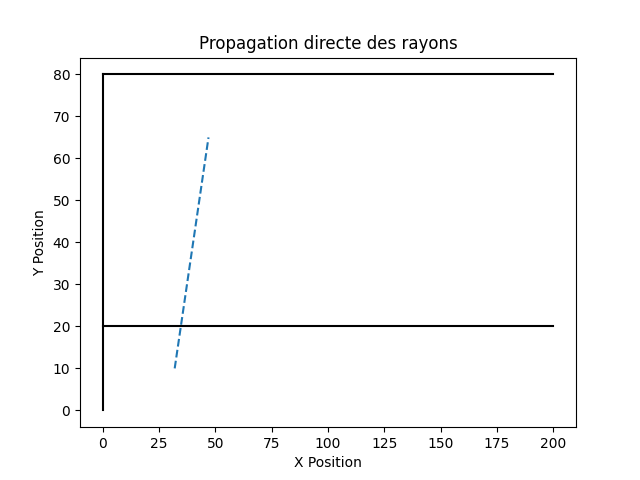
\includegraphics[width=\textwidth]{Pictures/propa_dir.png}
    \caption{Propagation directe \ref{fig:propd}}
    \label{fig:direct1}
\end{subfigure}
\hfill
\begin{subfigure}[b]{0.5\textwidth}
    \centering
    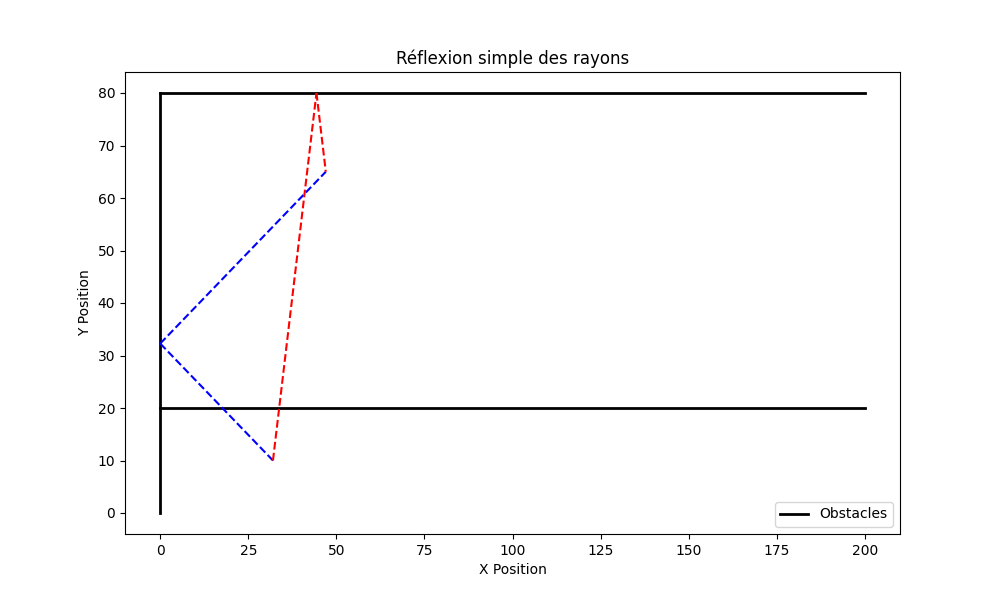
\includegraphics[width=\textwidth]{Pictures/simple_reflex.png}
    \caption{Réflexion simple \ref{refs}}
    \label{fig:simple_reflection}
\end{subfigure}

\begin{subfigure}[b]{0.45\textwidth}
    \centering
    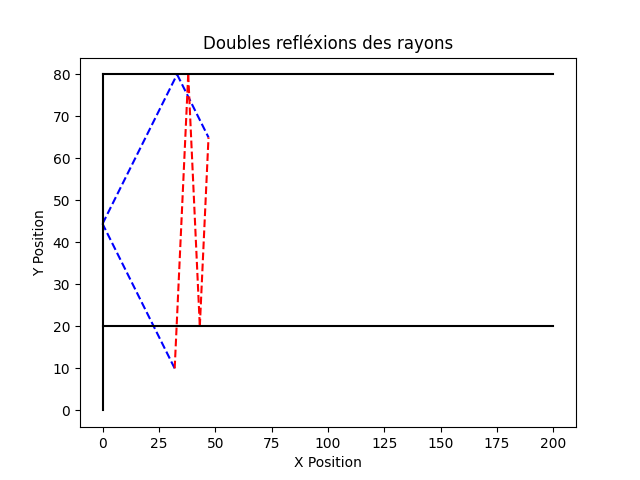
\includegraphics[width=\textwidth]{Pictures/double_reflex.png}
    \caption{Double réflexions \ref{refd}}
    \label{fig:double_reflection}
\end{subfigure}
\caption{Comparaison des différents types de propagation.}
\label{fig:ray_tracing}
\end{figure}

\subsubsection{Comparaison des Résultats}
Ci-dessous, le tableau comparant les valeurs obtenues manuellement avec celles de la simulation pour la propagation directe \ref{fig:direct1}.
\begin{table}[htbp]
\centering
\caption{Comparaison des résultats manuels et de simulation pour la propagation directe}
\label{tab:comparaison}
\begin{tabular}{@{}lcc@{}}
\toprule
\textbf{Paramètre} & \textbf{Valeur Manuelle} & \textbf{Valeur de Simulation} \\ \midrule
Champs Electrique (V/m) & $0.0037-0.0016j$ & $-0.0039994+3.8172944\times 10^{-5}j$ \\
Puissance reçue (W) &  $3.33 \times 10^{-10}$& $3.308468 \times 10^{-10}$ \\
Coefficient de transmission & $0.69+0.23j$ & $0.689195 + 0.237003j$ \\
Distance additionnelle parcourue (m) & $0.151$ & $0.151094$ \\
Angle d'incidence (degrés) & $15.2551$ & $15.255119$ \\
Angle de transmission (degrés) & $6.8796$ & $6.897650$ \\
Gamma perpendiculaire & $-0.3862+0.0165j$ & $-0.385931 + 0.016510j$ \\
$\gamma_m$ & $1.55+39.90j$ & $1.547482 + 39.872766j$ \\
Impédance du matériau $(\Omega)$ &$171.57+6.65j$& $171.683875 + 6.663138j$ \\
\bottomrule
\end{tabular}
\end{table} \\
La comparaison peut également être faite avec le cas à une réflexion pour le cas A (cas en bleu sur le graphe de la refléxion simple \ref{fig:simple_reflection}).
\begin{table}[htbp]
\centering
\caption{Comparaison des résultats manuels et de simulation pour la réflexion simple cas A}
\label{tab:comparaison_reflection}
\begin{tabular}{@{}lcc@{}}
\toprule
\textbf{Paramètre} & \textbf{Valeur Manuelle} & \textbf{Valeur de Simulation} \\ \midrule
Point d'impact ($P_r$) & $(0.0; 32.28)$ & $(0.0, 32.278481)$ \\
Angle d'incidence (degrés) & $34.8199$ & $34.84573$ \\
Angle de transmission (degrés) & $15.129$ & $15.1171208$ \\
Gamma perpendiculaire &$-0.4416+0.0156j$&$-0.441361+0.0156203j$\\
Coefficient de réflexion & $-0.334+0.225j$ & $-0.335708 + 0.225861j$ \\
Point d'impact ($P_t$) & $(17.64; 20)$ & $(17.636363;20)$ \\
Angle d'incidence (degré) & $55.1758$ & $55.1542665$ \\
Coefficient de transmission 1 (Émetteur $\rightarrow P_r$) & $0.539+0.023j$ & $0.537694 + 0.024983j$ \\
Distance additionnelle 1 (m) & $0.162$ & $0.161779$ \\
Coefficient de transmission 2 ($P_r \rightarrow$ récepteur) & $1+0j$ & $1.000000 + 0.000000j$ \\
Distance additionnelle 2 (m) & $0$ & $0.000000$ \\
Champs Electrique (V/m) & $-5.41\times 10^{-4}-4.57\times 10^{-4}j$ & $0.000441355+0.00055429153j $\\
Puissance reçue (W) &  $10.4 \times 10^{-12}$& $1.03829831227 \times 10^{-11}$ \\
\bottomrule
\end{tabular}
\end{table}\\
Pour les cas B à une reflexion et deux réflexion les résultats obtenus sont également ci dessous.\\
\begin{table}[H]
\centering
\caption{Comparaison des résultats manuels et de simulation pour les réflexions simple et doubles cas B}
\label{tab:comparaison_reflection}
\begin{tabular}{@{}lcc@{}}
\toprule
\textbf{Paramètre} & \textbf{Valeur Manuelle} & \textbf{Valeur de Simulation} \\ \midrule
cas B, réflexion simple & &\\ 
Champs Electrique (V/m) & $-4.52\times 10^{-4}-5.06\times 10^{-4}j$ & $0.000672792+0.00010809859j $\\
Puissance reçue (W) &  $9.5 \times 10^{-12}$& $9.6033123939 \times 10^{-12}$ \\
cas B, réflexion double & &\\ 
Champs Electrique (V/m) & $-7.86\times 10^{-5}-5.19\times 10^{-6}j$ & $-2.3403616\times 10^{-5} -7.614057941\times 10^{-5}j $\\
Puissance reçue (W) &  $0.1 \times 10^{-12}$& $1.3122870783 \times 10^{-13}$ \\
\bottomrule
\end{tabular}
\end{table}\\

Il est important de noter que les champs électriques sont différent pour les différents cas mais cela est dû à la grande variation de phase car l'émetteur est à $868.3 MHz$.\\
Après comparaison avec l'exercice 4.1 du syllabus du cours, les résultats sont similaire. Le simulateur est donc vérifié.
\section{Calcul du cas à 2 réflexions cas A}
Il a été demandé de calculer l'un des deux cas à 2 réflexions. Le cas ci dessous sera donc étudié.  
\begin{figure}[H]
    \centering
    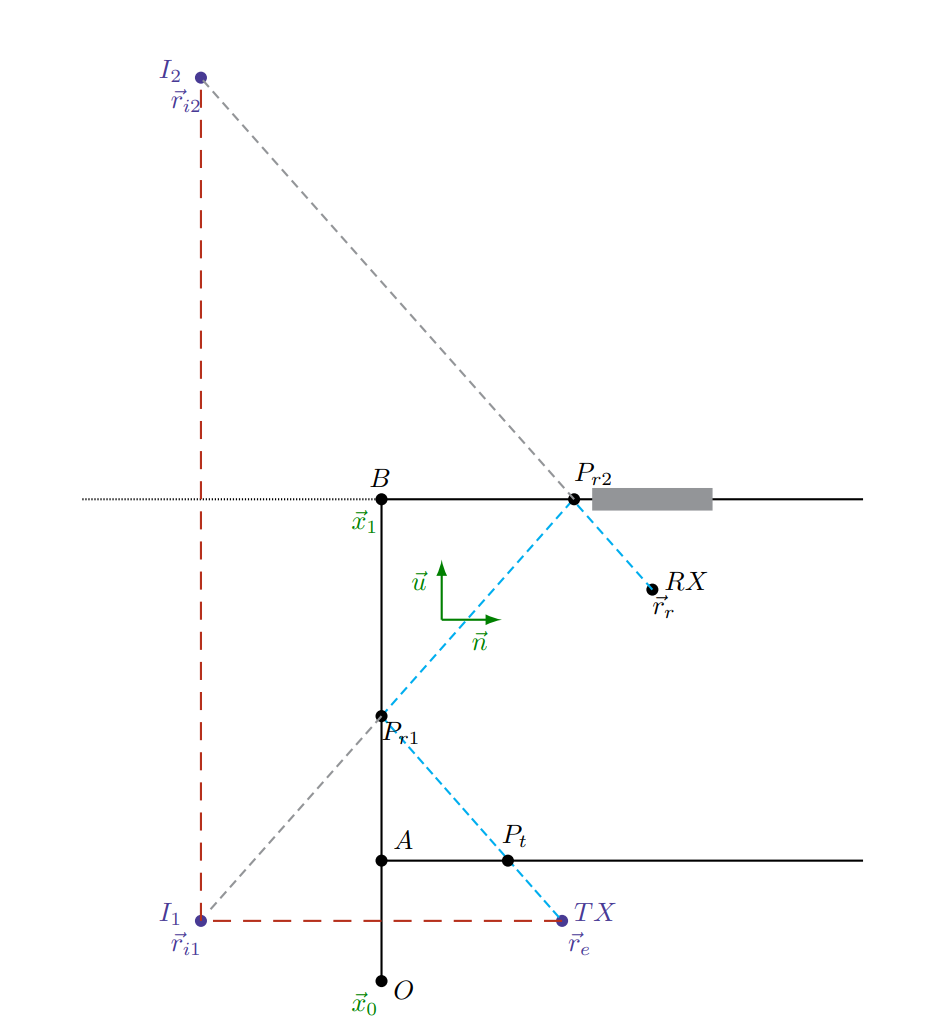
\includegraphics[width=0.58\textwidth]{Pictures/ex41.png}
    \caption{Cas A à 2 réflexions exercice 4.1}
    \label{fig:enter-label}
\end{figure}
\section*{Calcul des positions des points $Pr_2$, $Pr_1$ et $Pt$}

La position des antennes images est déterminée par symétrie orthogonale, avec les coordonnées suivantes pour les antennes images : $I_1 = (-32, 10)$ et $I_2 = (-32, 150)$. Les coordonnées des points $Pr_2$, $Pr_1$ et $Pt$ sont calculées comme suit :


\subsection*{Calcul de $Pr_2$}
$Pr_2$ est un point intermédiaire sur le trajet reliant $I_2$ à $RX$.Pour commencer, le vecteur a été calculé $\vec{v}_1$ entre $I_2$ et $RX$:
\[
\vec{v}_1 = (47 - (-32), 65 - 150) = (79, -85)
\]
La norme de $\vec{v}_1$ est calculée par :
\[
\|\vec{v}_1\| = \sqrt{79^2 + (-85)^2} = 116.0431
\]
Le vecteur unitaire de $\vec{v}_1$ est donc :
\[
\vec{u}_1 = \left(\frac{79}{116.0431}, \frac{-85}{116.0431}\right) = (0.6808, -0.7325)
\]
En posant la coordonnée y de $Pr_2$ à 80, en résolvant pour $\lambda$ dans l'équation suivante :
\[
(y; 80) = (-32; 150) + \lambda \vec{u}_1 \implies \lambda = \frac{80 - 150}{-0.7325} = 95.5631
\]
D'où :
\[
x = -32 + 95.5631 \times 0.6808 = 33.0593
\]
Ainsi, $Pr_2 = (33.0593, 80)$.

\subsection*{Calcul de $Pr_1$}
Pour calculer $Pr_1$, reliant $I_1$ à $Pr_2$, le vecteur $\vec{v}_2$ est :
\[
\vec{v}_2 = (33.0593 - (-32), 80 - 10) = (65.0593, 70)
\]
Sa norme est :
\[
\|\vec{v}_2\| = \sqrt{(65.0593)^2 + 70^2} = 95.5652
\]
Le vecteur unitaire est :
\[
\vec{u}_2 = \left(\frac{65.0593}{95.5652}, \frac{70}{95.5652}\right) = (0.6808, 0.7325)
\]
Pour une coordonnée x de $Pr_1$ à 0, j'ai trouvé $\lambda$ :
\[
(0; y) = (-32; 10) + \lambda \vec{u}_2 \implies \lambda = \frac{0 - (-32)}{0.6808} = 47.0035
\]
Donc :
\[
y = 10 + 47.0035 \times 0.7325 = 44.4301
\]
Finalement, $Pr_1 = (0, 44.4301)$.

\subsection*{Calcul de $Pt$}
La méthode similaire est appliquée pour $Pt$. Le vecteur $\vec{v}_3$ et sa norme sont :
\[
\vec{v}_3 = (0 - 32, 44.4301 - 10) = (-32, 34.4301), \quad \|\vec{v}_3\| = \sqrt{(-32)^2 + (34.4301)^2} = 47.0046
\]
Le vecteur unitaire est :
\[
\vec{u}_3 = \left(\frac{-32}{47.0046}, \frac{34.4301}{47.0046}\right) = (-0.6808, 0.7325)
\]
Pour une coordonnée y de $Pt$ à 20, $\lambda$ est résolu comme suit :
\[
(x; 20) = (32; 10) + \lambda \vec{u}_3 \implies \lambda = \frac{20 - 10}{0.7325} = 13.6519
\]
Ce qui donne :
\[
x = 32 + 13.6519 \times (-0.6808) = 22.7058
\]
Ainsi, $Pt = (22.7058, 20)$.

\section*{Coefficients de réflexion et transmission}

Le rayon subit une transmission et deux réflexions au cours de son trajet. Il est donc nécessaire de calculer deux coefficients de réflexion ainsi qu'un coefficient de transmission.

\subsection*{Calcul du coefficient $\Gamma_2$}
Le vecteur normal au point $Pr_2$ est donné par $(0, -1)$. La projection de $\vec{v}_1$ normé sur ce vecteur normal donne $\cos \theta_i = \langle (0.6808, -0.7325), (0, -1) \rangle = 0.7325$. Ainsi, $\sin \theta_i$ est obtenu par:
\[
\sin \theta_i = \sqrt{1 - 0.7325^2} = 0.6808.
\]
Le $\sin \theta_t$ est déterminé par la loi de Snell:
\[
\sin \theta_t = \sqrt{\frac{1}{\epsilon_r}} \sin \theta_i = \sqrt{\frac{1}{4.8}} \times 0.6808 = 0.3107 \quad \text{et donc} \quad \cos \theta_t = \sqrt{1 - 0.3107^2} = 0.9505.
\]
La distance de pénétration $s$ est calculée comme:
\[
s = \frac{l}{\cos \theta_t} = \frac{0.15}{0.9505} = 0.1578.
\]
Le coefficient de réflexion $\Gamma_{\perp}$ est alors:
\[
\Gamma_{\perp} = \frac{Z_m \cos \theta_i - Z_0 \cos \theta_t}{Z_m \cos \theta_i + Z_0 \cos \theta_t} = \frac{(171.57 + j6.65) \times 0.7325 - 377 \times 0.9505}{(171.57 + j6.65) \times 0.7325 + 377 \times 0.9505} = -0.4805 + j0.0149.
\]
Avec ces valeurs, $\Gamma_2$ est calculé par:
%\Gamma_m(\theta_i) = \Gamma_{\perp}(\theta_i) - \frac{(1 - \Gamma^2_{\perp}(\theta_i)) \Gamma_{\perp}(\theta_i) e^{-2\gamma_m s} e^{j\beta2s \sin \theta_t \sin \theta_i}}{1 - \Gamma^2_{\perp}(\theta_i) e^{-2\gamma_m s} e^{j\beta2s \sin \theta_t \sin \theta_i}}

\[
\Gamma_2 =  \Gamma_{\perp}(\theta_i) -(1 - \Gamma^2_{\perp}(\theta_i)) \frac{ \Gamma_{\perp}(\theta_i) e^{-2\gamma_m s} e^{j\beta2s \sin \theta_t \sin \theta_i}}{1 - \Gamma^2_{\perp}(\theta_i) e^{-2\gamma_m s} e^{j\beta2s \sin \theta_t \sin \theta_i}} = -0.4188 + 0.2462j.
\]

\subsection*{Calcul du coefficient $\Gamma_1$}
Pour le deuxième calcul, je projete $\vec{v}_2$ normé sur la normale $(1, 0)$, donnant $\cos \theta_i = 0.6808$. Les calculs suivants utilisent cette valeur:
\[
\sin \theta_i = 0.7325, \quad \sin \theta_t = 0.3343, \quad \cos \theta_t = 0.9425, \quad s = 0.1591.
\]
Le coefficient de réflexion perpendiculaire $\Gamma_a$ est:
\[
\Gamma_{a,\perp} = \frac{Z_m \cos \theta_i - Z_0 \cos \theta_t}{Z_m \cos \theta_i + Z_0 \cos \theta_t} = \frac{(171.57 + j6.65) \times 0.6808 - 377 \times 0.9425}{(171.57 + j6.65) \times 0.6808 + 377 \times 0.9425} = -0.5050 + j0.0144.
\]
Ainsi, $\Gamma_1$ est:
\[
\Gamma_1 = \Gamma_{\perp}(\theta_i) -(1 - \Gamma^2_{\perp}(\theta_i)) \frac{ \Gamma_{\perp}(\theta_i) e^{-2\gamma_m s} e^{j\beta2s \sin \theta_t \sin \theta_i}}{1 - \Gamma^2_{\perp}(\theta_i) e^{-2\gamma_m s} e^{j\beta2s \sin \theta_t \sin \theta_i}}= -0.4710 + 0.2518j.
\]

\subsection*{Calcul du coefficient de transmission $T_1$}
Le $\cos \theta_i$ pour le point $Pt$ est $0.7325$. En dérivant $\sin \theta_i$, $\sin \theta_t$, et $\cos \theta_t$ comme précédemment. Le coefficient de réflexion perpendiculaire $\Gamma_b$ est:
\[
\Gamma_{b,\perp} = \frac{Z_m \cos \theta_i - Z_0 \cos \theta_t}{Z_m \cos \theta_i + Z_0 \cos \theta_t} = \frac{(171.57 + j6.65) \times 0.7325 - 377 \times 0.1578}{(171.57 + j6.65) \times 0.7325 + 377 \times 0.1578} = -0.5082 + j0.0144.
\]
Le coefficient de transmission $T_1$ est alors calculé par:
\[
T_1 = \frac{ (1 - \Gamma^2_{\perp}(\theta_i)) e^{-2\gamma_m s}}{1 - \Gamma^2_{\perp}(\theta_i) e^{-2\gamma_m s} e^{j\beta2s \sin \theta_t \sin \theta_i}} = 0.6295 + 0.0890j.
\]

%\section*{Calcul de la distance totale parcourue par le rayon et puissance reçue au récepteur}

%\subsection*{Distance totale parcourue par le rayon}
%La distance totale parcourue par le rayon est calculée en additionnant les distances entre les différents points du trajet du rayon de $TX$ à $RX$ :
%\begin{align*}
%\text{Trajet } TX/Pt & : \sqrt{(22.7058 - 32)^2 + (20 - 10)^2} = 13.6522, \\
%\text{Trajet } Pt/Pr1 & : \sqrt{(0 - 22.7058)^2 + (44.4301 - 20)^2} = 33.3524, \\
%\text{Trajet } Pr2/Pr1 & : \sqrt{(33.0593 - 0)^2 + (80 - 44.4301)^2} = 48.5606, \\
%\text{Trajet } PRX/Pr2 & : \sqrt{(47 - 33.0593)^2 + (65 - 80)^2} = 20.4779.
%\end{align*}
%La distance totale est donc de $116.0431$ mètres. Cette distance peut également être vérifiée en calculant directement la distance entre la dernière antenne image $I_2$ et le récepteur $RX$ :
%\[
%\sqrt{(47 - (-32))^2 + (65 - 150)^2} = 116.0431 \text{ mètres}.
%\]

\subsection{Calcul du champ et de la puissance reçue au récepteur}
La valeur du champ électrique reçu, $E_n$, est calculée à partir des coefficients de transmission et de réflexion, et est donnée par :
\[
E_n = \Gamma_1 \Gamma_2 T_1 \sqrt{60 G_{TX} P_{TX}} \frac{e^{-j \beta d_n}}{d_n}
\]
où $\Gamma_1 = -0.4710 + 0.2518j$, $\Gamma_2 = -0.4188 + 0.2462j$, $T_1 = 0.6295 + 0.0890j$, et $d_n = 116.0431$(norme de $v_1$). En calculant $\Gamma_1 \Gamma_2 T_1$ :
\[
\Gamma_1 \Gamma_2 T_1 = (-0.4710 + 0.2518j)(-0.4188 + 0.2462j)(0.6295 + 0.0890j) = 0.1059 - 0.1273j
\]
Ainsi, en substituant les valeurs et calculant $\beta$ à partir de la fréquence $f = 868.3$ MHz :
\[
\beta = \frac{2\pi f}{c} = \frac{2\pi \times 868.3 \times 10^6}{3 \times 10^8} \quad (\text{avec } c \text{ la vitesse de la lumière})
\]
La valeur de $E_n$ obtenue est :

\[
E_n = (0.0159 - 0.1273j) \sqrt{60 \times 1.64 \times 10^{-3}} \frac{e^{-j \beta \times 116.0431}}{116.0431} 
\]
\[
E_n \approx 4.4519 \times 10^{-4} - 2.1816 \times 10^{-5}j
\]
La puissance totale reçue, $P_{RX}$, est ensuite calculée par :
\[
P_{RX} = \frac{\lambda^2}{8\pi^2 R_a} \|E_n\|^2 = \left(\frac{3 \times 10^8}{868.3 \times 10^6}\right)^2 \frac{1}{8\pi^2 \times 73} \|4.4519 \times 10^{-4} - 2.1816 \times 10^{-5}j\|^2
\]
\[
P_{RX} \approx 4.1145 \times 10^{-12} \text{ Watts} \quad \text{ou} \quad P_{RX} \approx -83.8568 \text{ dBm}
\]
\begin{table}[htbp]
\centering
\caption{Comparaison des résultats manuels et simulés pour la réflexion doubles cas A}
\label{tab:double_reflection_comparison}
\begin{tabular}{@{}lcc@{}}
\toprule
\textbf{Paramètre} & \textbf{Valeur Manuelle} & \textbf{Valeur de Simulation} \\ \midrule
Point d'impact 1 & $(0, 44.4301)$ & $(0.0, 44.4304)$ \\
Point d'impact 2 & $(33.0593, 80)$ & $(33.059, 80.0)$ \\
Angle d'incidence($\Gamma_1$) $\theta_{i1}$ (degrés) & $47.09381$ & $47.09525256$ \\
Angle de transmission $\theta_t1$ (degrés) & $19.531$ & $19.531971$ \\
Angle d'incidence($\Gamma_2$) $\theta_{i2}$ (degrés) & $42.9031$ & $42.90474743$ \\
Angle de transmission $\theta_t2$ (degrés) & $18.103$ & $18.1034009$ \\
Coefficient de réflexion $\Gamma_{\perp1}$ & $(-0.5050+0.0144j)$ & $(-0.504537+0.014614j)$ \\
Coefficient de réflexion $\Gamma_{\perp2}$ & $(-0.4805+0.0149j)$ & $(-0.480021+0.014929j)$ \\
Coefficients de transmission 1 & $(0.6295+0.0890j)$ & $(0.6289223+0.0918245j)$ \\
Coefficients de transmission 2 & $1.0$ & $1.0$ \\
Coefficients de transmission 3 & $1.0$ & $1.0$ \\
Distance totale (mètres) & $116.0431$ & $116.043095$ \\
Coefficient total & $(0.1059-0.1273j)$ & $(0.1064106-0.1273762j)$ \\
Champ électrique (V/m)& $4.4519 \times 10^{-4} - 2.1816 \times 10^{-5}j$ & $(3.05628 \times 10^{-5} - 0.0004476j)$  \\
Puissance reçue (W)&$4.1145 \times 10^{-12}$ & $4.16327 \times 10^{-12}$  \\

\bottomrule
\end{tabular}
\end{table}

\chapter{Resultat et Optimisation}
Après validation du simulateur, l'implémentation des caractéristiques spécifiques du projet a été réalisée, telles que l'environnement de simulation, la fréquence des ondes utilisées et les conditions spécifiques du projet détaillées dans le cahier des charges. Le simulateur a été configuré pour une fréquence de 60 GHz, correspondant à la norme IEEE 802.11ay pour le Wi-Fi, et a été simulé en présence et en absence de l'ascenseur. \footnote{Tous les graphes de ce chapitre sont en grande taille en Annexe A.}


\section{Configuration initiale}
L'environnement de simulation comprend plusieurs obstacles représentant les murs internes et externes d'un appartement. Ces obstacles ont été modélisés avec des propriétés matérielles spécifiques, telles que la permittivité et la conductivité, qui influencent la réflexion et la transmission des ondes. Un émetteur unique a été placé initialement en un point imposé de l'appartement, précisément à la position (9,4m ; -7m).
\begin{figure}[H]
    \centering
    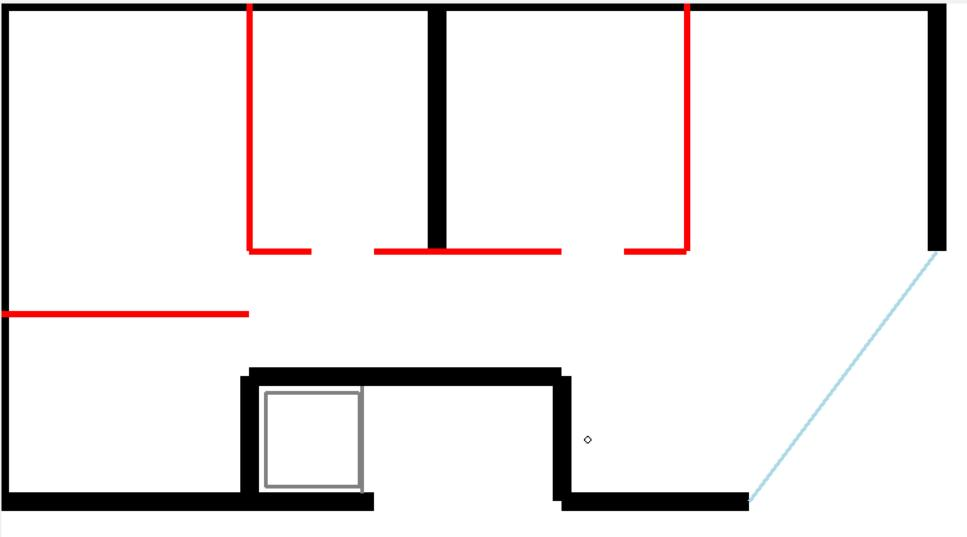
\includegraphics[width=0.6\textwidth]{Pictures/plan appart.jpeg}
    \caption{implémentation de l'appartement}
    \label{appart}
\end{figure}

\subsubsection{Résultats}
Les résultats de cette première simulation ont montré des zones de couverture inégales, avec des diminutions notables de puissance dans les zones éloignées de l'émetteur ou situées derrière des obstacles à forte atténuation. Seulement une partie de la maison est couverte, que ce soit avec ou sans l'ascenseur. Pour la situation avec ascenseur, la puissance moyenne dans tout l'appartement\footnote{Pour le calcul de la moyenne,l'emplacement de l'ascenseur fait partie de l'appartement, qu'il soit à l'étage ou non} est de $-69,65$ dBm. Ensuite, pour trouver le débit binaire à chaque endroit, la linéarité entre la puissance et le débit binaire a été exploitée en faisant une interpolation linéaire pour les valeurs comprises entre $]-90;-40[$ dBm. L'équation linéaire est de type :

\begin{equation}
    y_{Mbps}= (P_{dBm}+90)\times (\frac{39950}{50}) +50
\end{equation} 

Les valeurs supérieur à -40 dBm ont directement été associés à $40000 \frac{Mb}{s}$ et celle inférieur à -90 dBm à $50 \frac{Mb}{s}$.
Les heatmaps associées sont ci dessous\footnote{Il a été décidé d'afficher les heatmaps pour une résolution de $0,2m \times 0,2m$.}.

\begin{figure}[H]
\centering
\begin{subfigure}[b]{0.49\textwidth}
    \centering
    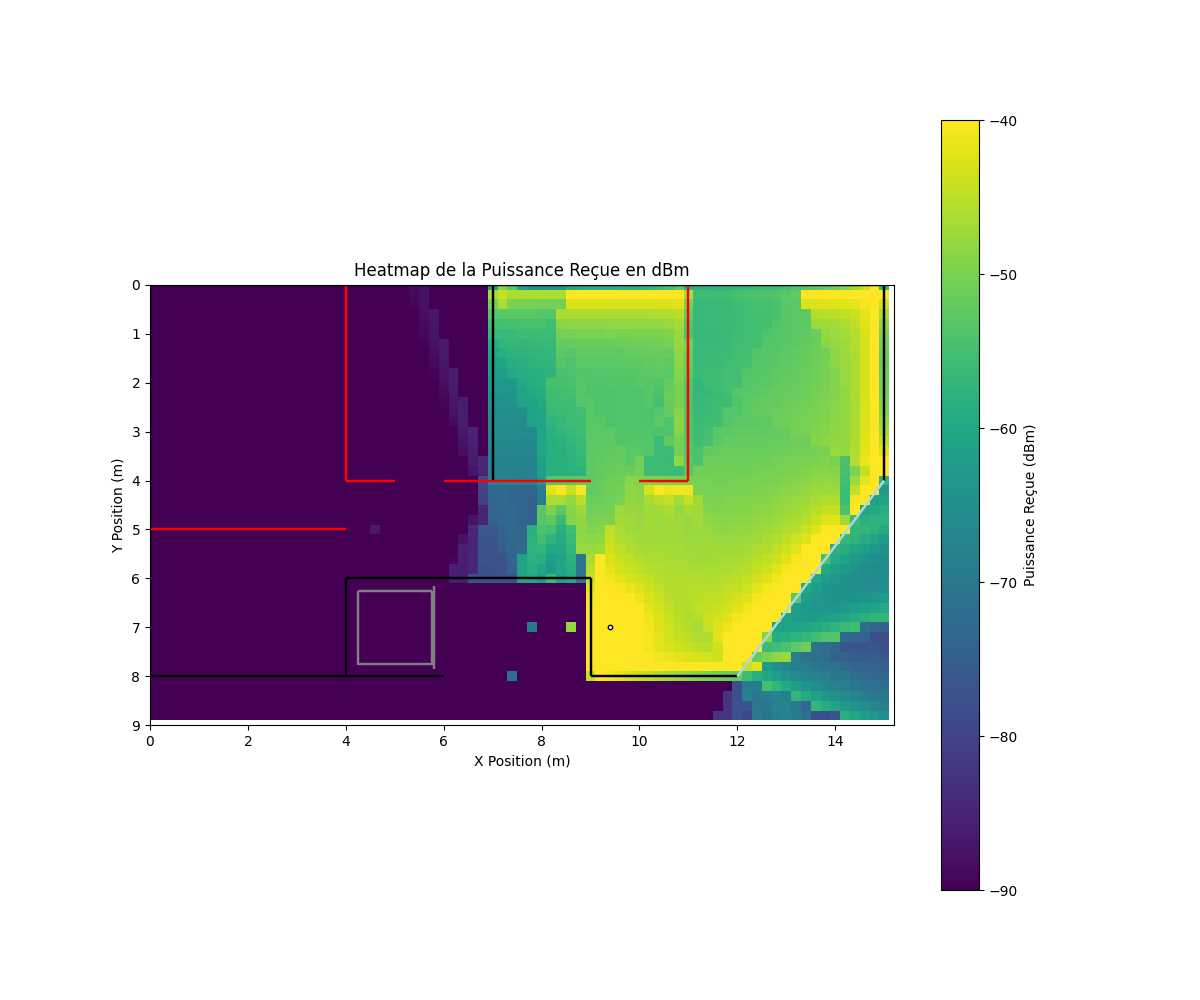
\includegraphics[width=\textwidth]{Pictures/dBm.png}
    \caption{Heatmap puissance (dBm)\ref{dbmbasea}}
    \label{fig:direct}
\end{subfigure}
\hfill
\begin{subfigure}[b]{0.49\textwidth}
    \centering
    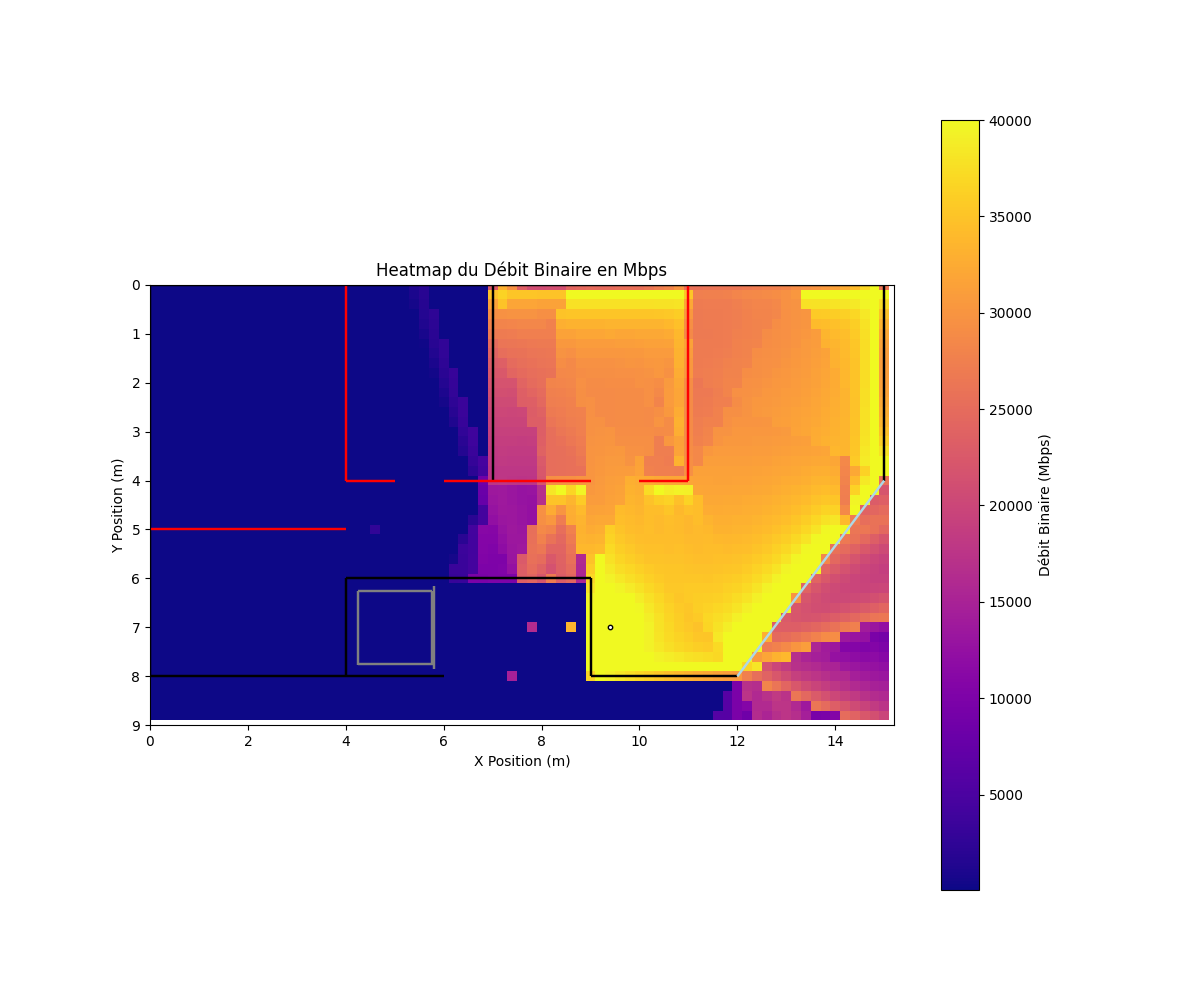
\includegraphics[width=\textwidth]{Pictures/mbps.png}
    \caption{Heatmap débit binaire (Mb/s)\ref{mbpsbasea}}
    \label{fig:}
\end{subfigure}
\caption{Différentes heatmaps du scénario de base avec ascenseur }
\label{fig:ray_tracing}
\end{figure}

Ensuite, le cas où l'ascenseur n'est pas à l'étage a été pris en compte. On remarque ci-dessous \ref{okemec} que ce scénario est similaire à celui avec ascenseur, car la puissance moyenne dans l'appartement est identique. Cela est dû au mauvais placement de l'antenne.

\begin{figure}[H]
\centering
\begin{subfigure}[b]{0.48\textwidth}
    \centering
    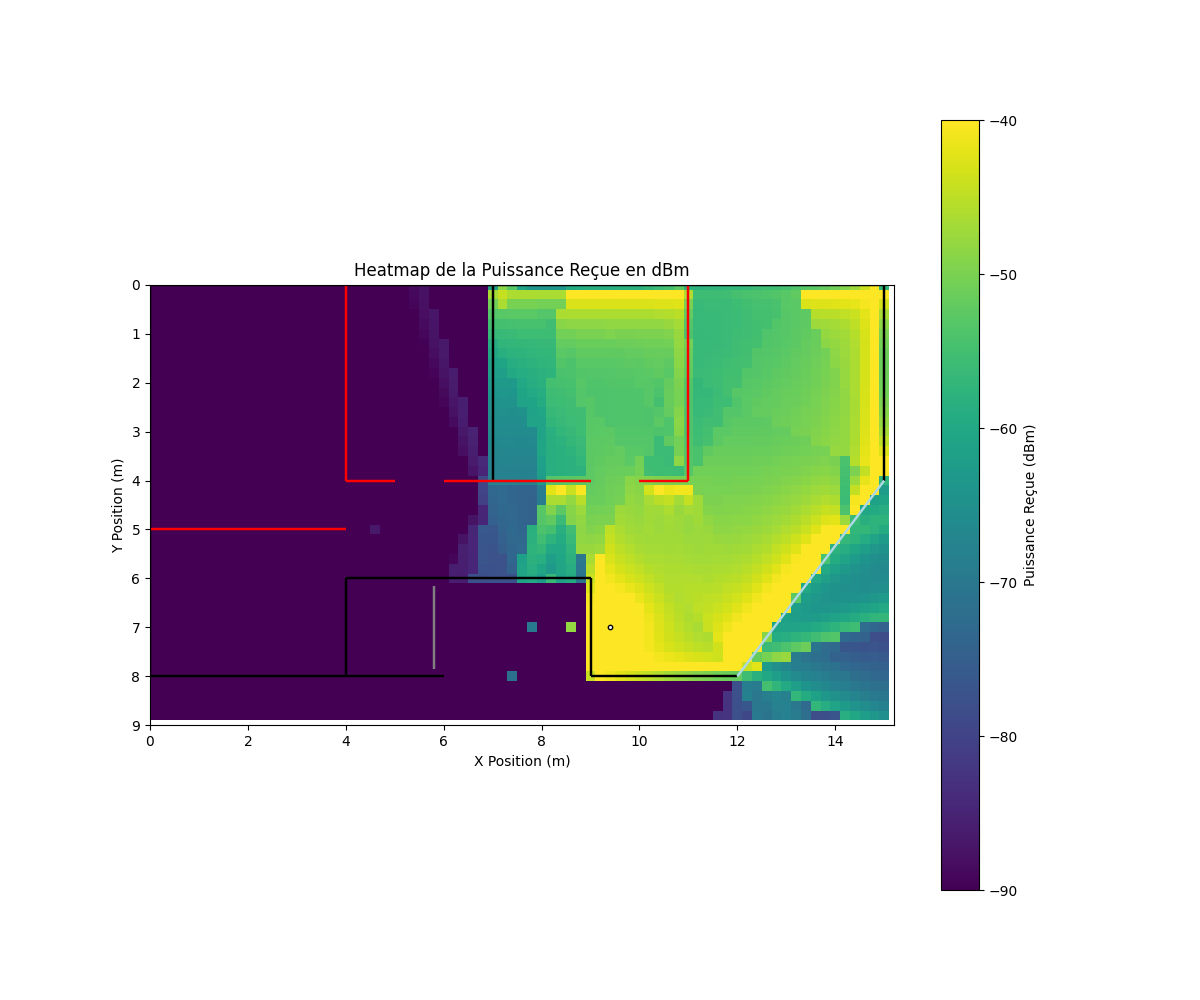
\includegraphics[width=\textwidth]{Pictures/bpmsa.png}
    \caption{Heatmap puissance (dBm)\ref{dbmbasesa}}
    \label{fig:}
\end{subfigure}
\hfill
\begin{subfigure}[b]{0.48\textwidth}
    \centering
    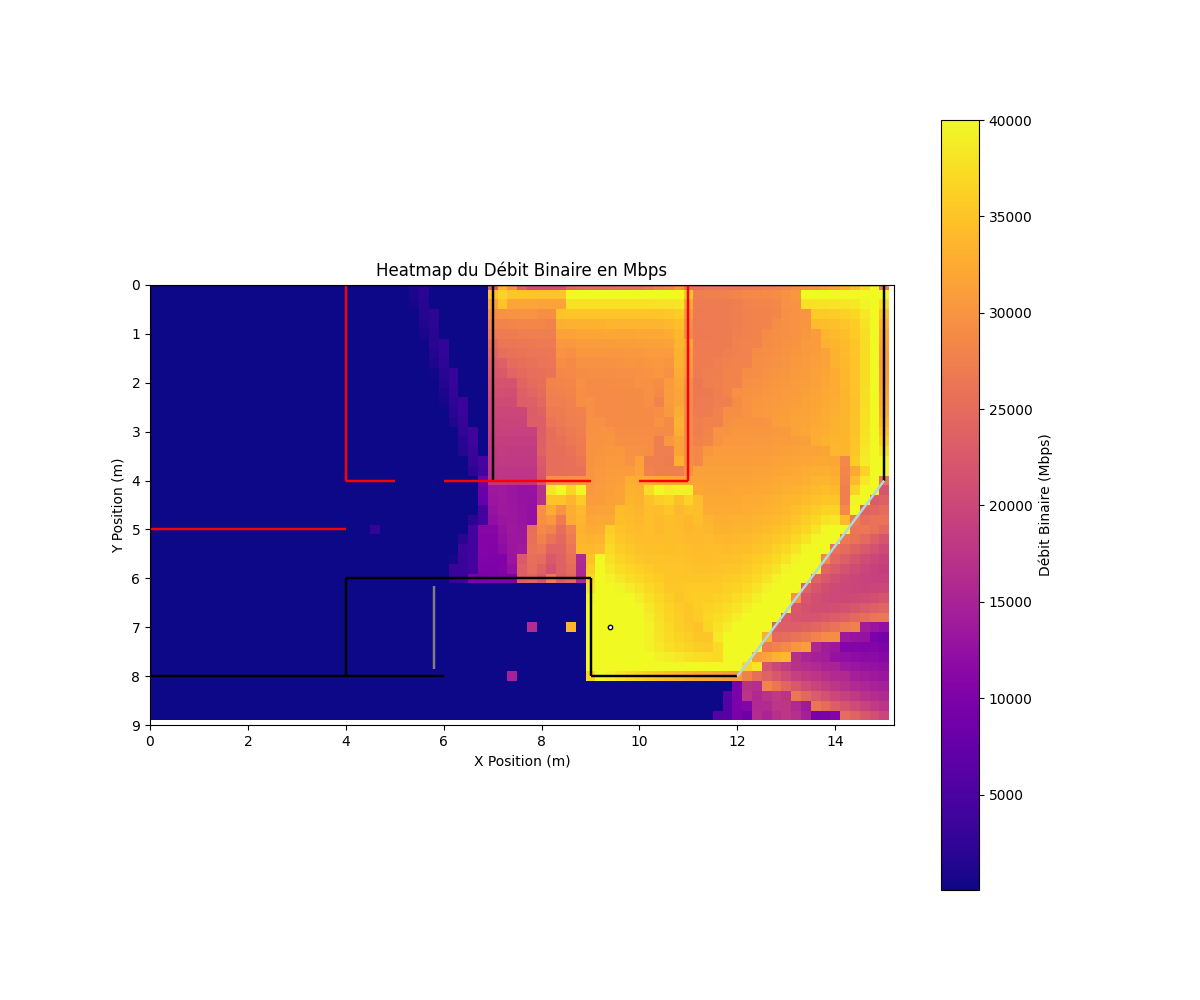
\includegraphics[width=\textwidth]{Pictures/mbpssa.png}
    \caption{Heatmap débit binaire (Mb/s)\ref{mbpsbasesa}}
    \label{fig:}
\end{subfigure}
\caption{Différentes heatmaps du scénario de base sans ascenseur }
\label{okemec}
\end{figure}
\section{Optimisation et Couverture de l'Appartement}

\subsection*{Exploitation de l'Architecture Multicœur}
L'ordinateur possède un processeur Intel Core i7, avec ses multiples cœurs, permettant une exécution en parallèle efficace des calculs. L'implémentation utilise \texttt{ProcessPoolExecutor} du module \texttt{concurrent.futures} pour distribuer les tâches de calcul de la puissance reçue à différents cœurs, réduisant ainsi le temps total d'exécution de manière significative.

\subsection{Optimisation par GPU}
L'ordinateur possède aussi une carte NVIDIA GeForce RTX, équipée de l'architecture Turing, permettant une accélération significative des tâches graphiques. Cependant, cela demanderait une réécriture non négligeable du code. Par souci de temps et en raison des bons résultats obtenus, l'utilisation de la carte graphique n'a pas été prise en compte dans le code.

\subsection{Automatisation de l'Optimisation des Emplacements des Émetteurs}
L'algorithme d'optimisation des emplacements des émetteurs utilise une grille de recherche exhaustive combinée à la parallélisation pour identifier la position optimale des émetteurs dans l'appartement. Dans un premier temps, une résolution plus grande est utilisée pour centraliser la position de l'émetteur, puis une résolution plus petite est appliquée en utilisant un système de cache pour éviter la redondance des calculs identiques. Cela permet d'éviter le calcul des zones qui ne sont pas à considérer. Cette méthode, en exploitant pleinement les ressources multicœurs du processeur Intel Core i7, réduit les délais de calcul. Cela a été réalisé pour l'emplacement de un et deux émetteurs.

\subsection{Résultats obtenus}
Grâce à ces optimisations, les heatmaps sont créées en seulement 6 à 14 secondes\footnote{Cela dépend si l'ordinateur est en charge ou non et si d'autres applications sont actives en arrière-plan} plutôt qu'en 8 à 11 minutes dans le cas non optimisé. Pour optimiser, l'ascenseur n'a pas été pris en compte. Il a été jugé que maximiser la couverture dans un ascenseur n'est pas pertinent.
\subsubsection{Couverture de l'appartement avec un émetteur}
La fonction d'optimisation pour un émetteur a permis de trouver la position optimale suivante : (7, -4.5). Cette position couvre tout l'appartement et permet une puissance moyenne de $-53,18$ dBm avec l'ascenseur à l'étage et une puissance moyenne de $-53,08$ dBm sans l'ascenseur à l'étage.\footnote{Les heatmaps de débit binaire sont également en annexe}

\begin{figure}[H]
\centering
\begin{subfigure}[b]{0.48\textwidth}
    \centering
    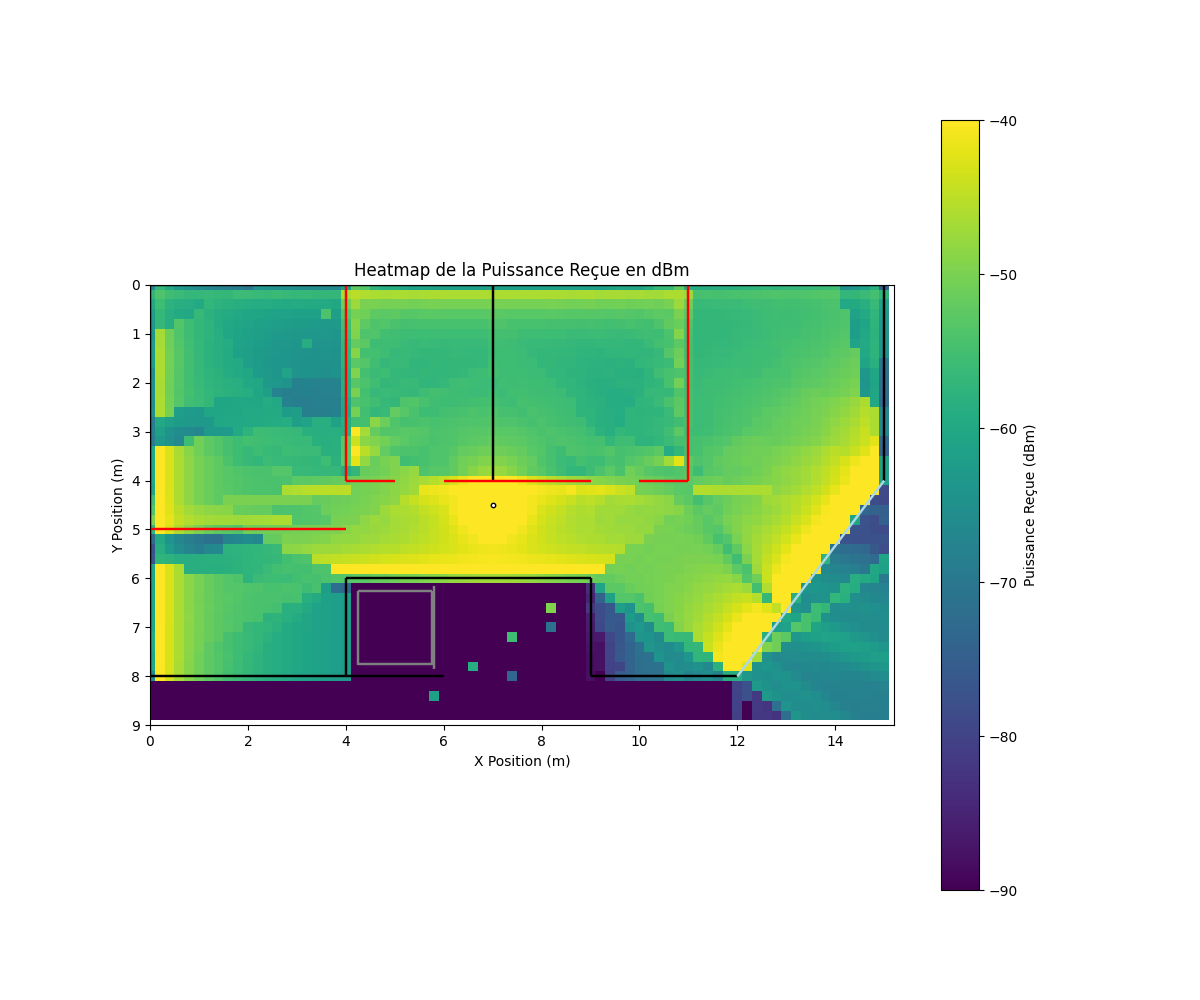
\includegraphics[width=\textwidth]{Pictures/opt1bpma.png}
    \caption{Heatmap puissance (dBm) avec ascenseur\ref{opti1adbm}}
    \label{fig:}
\end{subfigure}
\hfill
\begin{subfigure}[b]{0.48\textwidth}
    \centering
    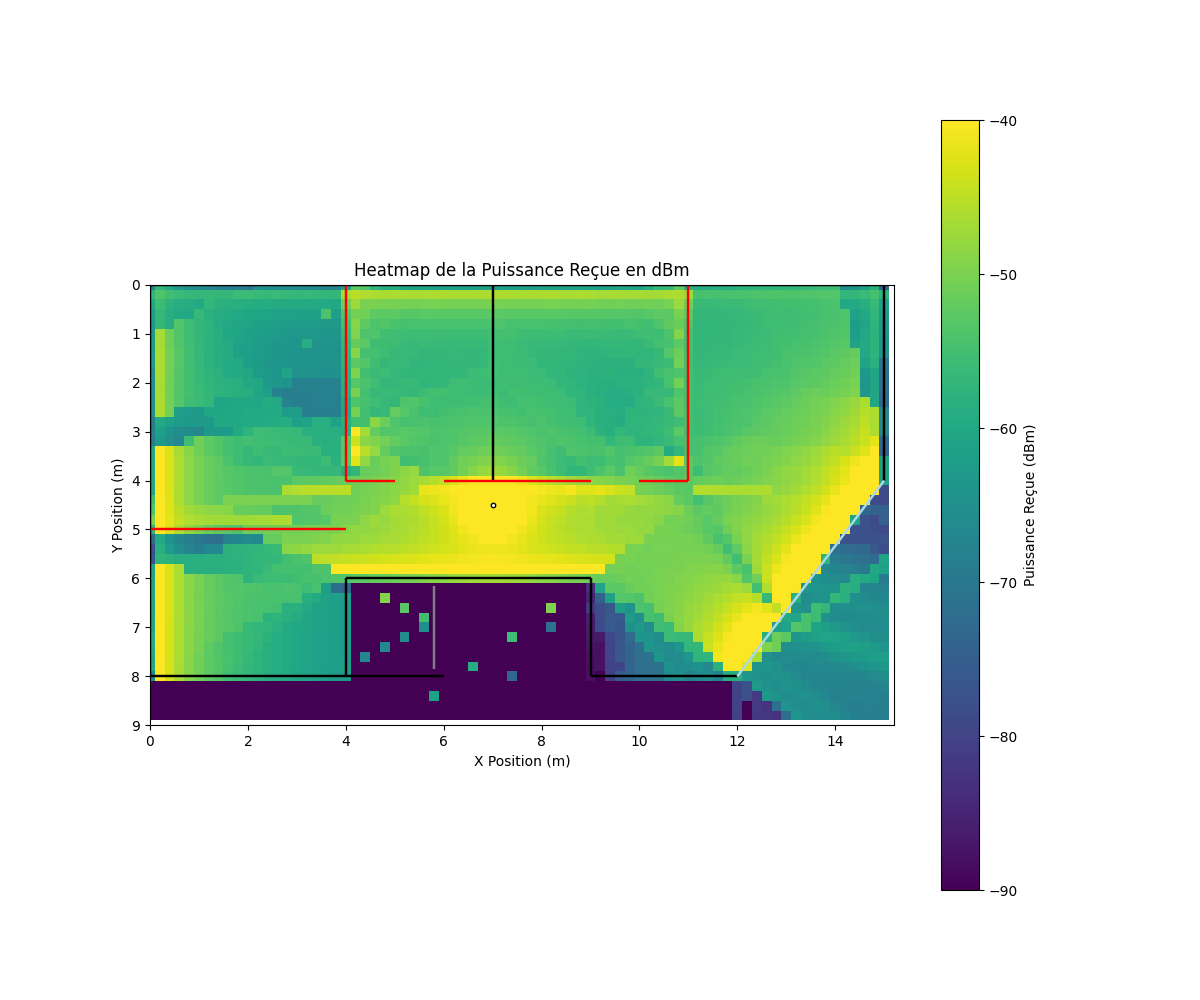
\includegraphics[width=\textwidth]{Pictures/opt1bpm.png}
    \caption{Heatmap puissance (dBm) sans ascenseur\ref{opti1dbm}}
    \label{fig:}
\end{subfigure}
\caption{Heatmaps de l'optimisation à 1 émetteur avec et sans ascenseur }
\label{okem}
\end{figure}
\subsubsection{Couverture de l'appartement à deux émetteurs}
La fonction d'optimisationà 2 émetteurs a trouvé comme positions optimales (2.5,-2.5) et (10.5,-4.5).Elles assurent une couverture totale de l'appartement dans les deux cas, que l'ascenseur soit à l'étage ou non. La puissance moyenne dans tout l'appartement reste identique dans les deux cas et est  $-48.97$ dBm. %Cependant, avoir une antenne dans sa chambre peut être dérangeant. Une optimisation sans les chambres a été faite et les positions revenues sont (4.5,-5) et (2.5,-2.5) avec une puissance moyenne de $-49.00$ dBm. Les heatmaps sont en annexe 
\begin{figure}[H]
\centering
\begin{subfigure}[b]{0.48\textwidth}
    \centering
    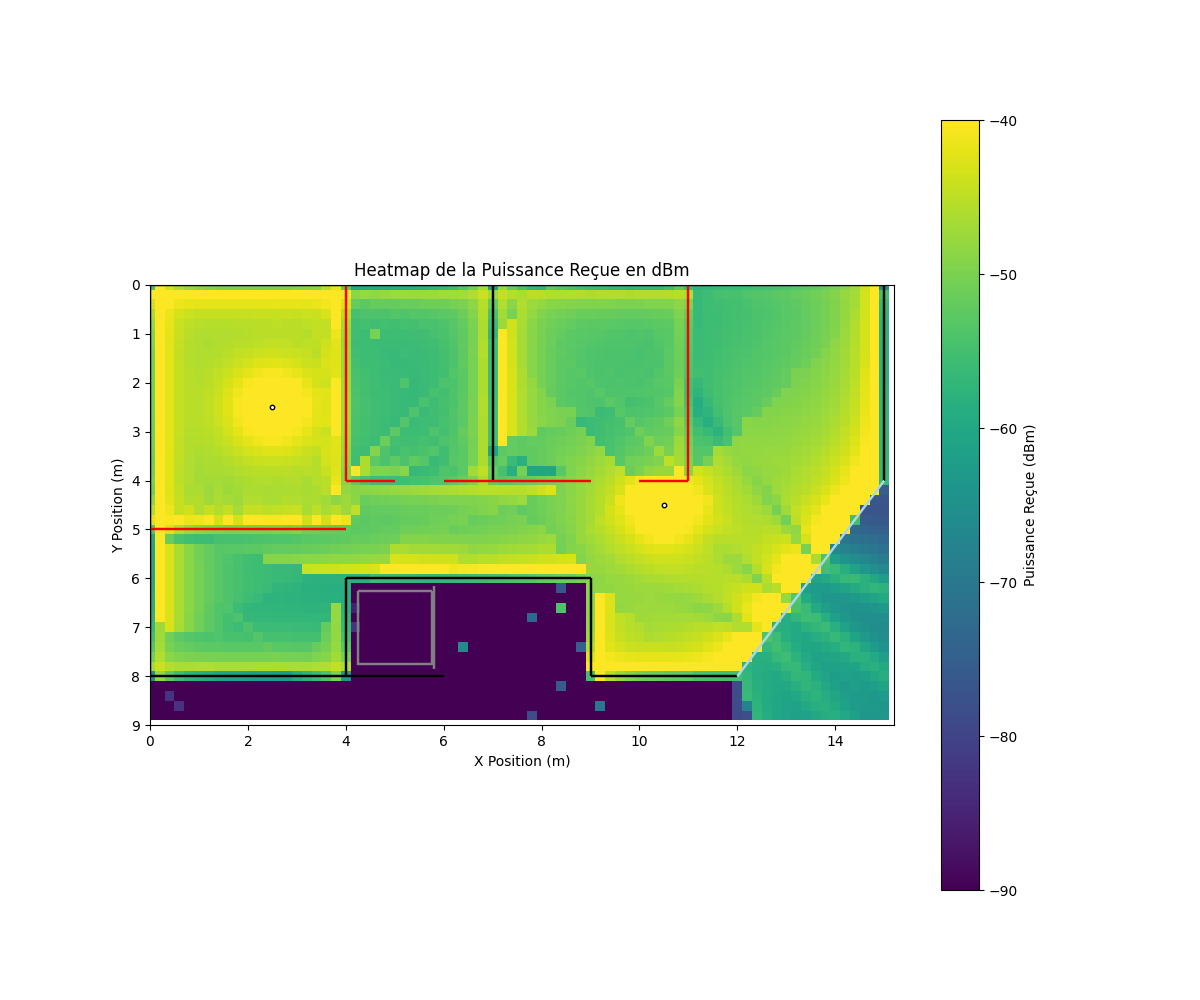
\includegraphics[width=\textwidth]{Pictures/opti2dbma.png}
    \caption{Heatmap puissance (dBm) avec ascenseur\ref{opti2dbma}}
    \label{fig:}
\end{subfigure}
\hfill
\begin{subfigure}[b]{0.48\textwidth}
    \centering
    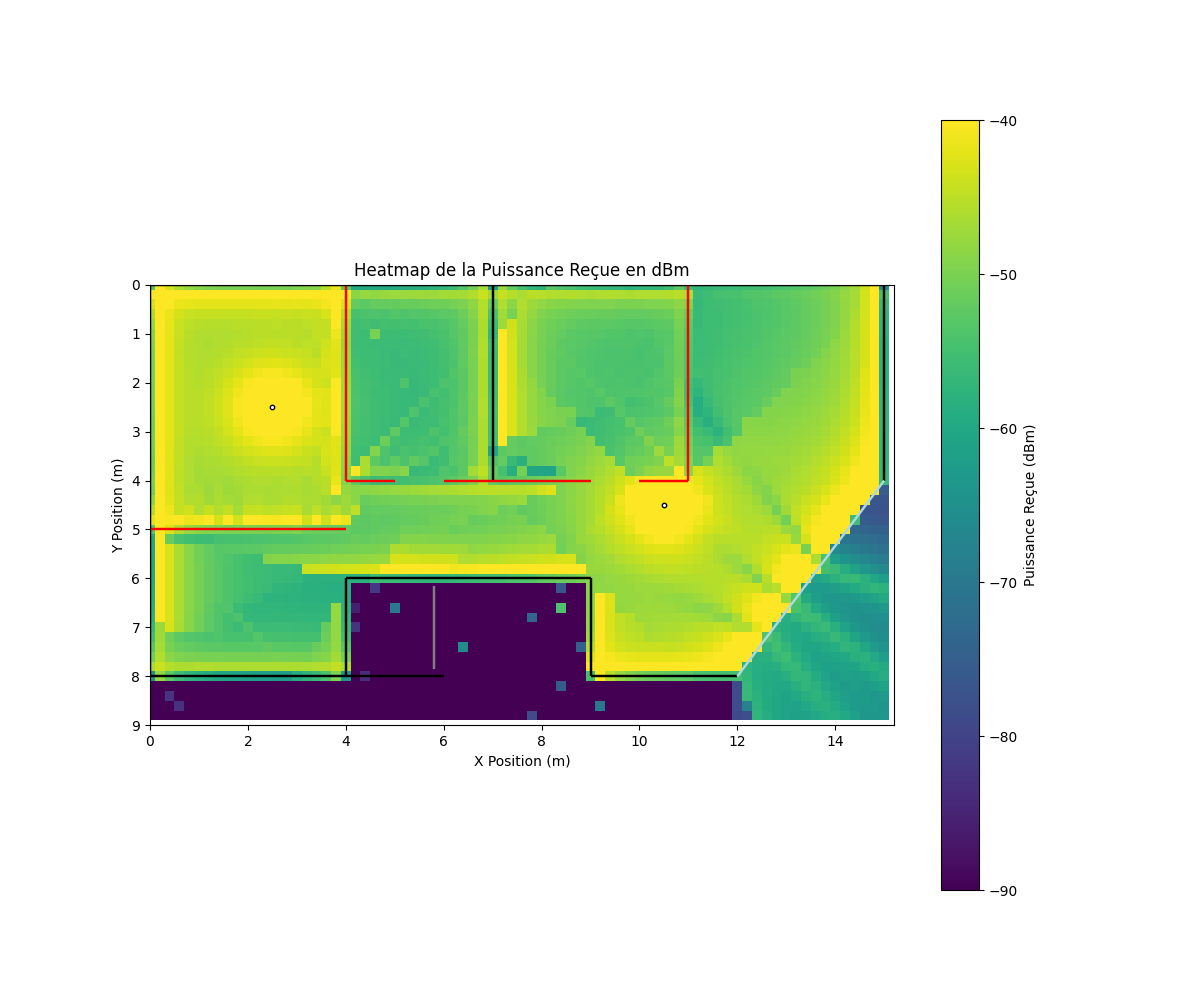
\includegraphics[width=\textwidth]{Pictures/opti2dbm.png}
    \caption{Heatmap puissance (dBm) sans ascenseur \ref{opti2dbm}}
    \label{fig:}
\end{subfigure}
\caption{Heatmaps de l'optimisation à 2 émetteurs avec et sans ascenseur }
\label{okem}
\end{figure}

L'optimisation de la position de l'émetteur est essentielle pour assurer une couverture totale de l'appartement. Il a été possible de passer de $-69,65$ dBm à $-53,08$ dBm en plaçant le même émetteur à une position optimale. % La différence de puissance de $-18,11$ dBm est considérable.
Il est également possible d'améliorer cette puissance moyenne en ajoutant des émetteurs, mais dans un cas réel cela coûterait également plus cher. Lorsque l'ascenseur est à l'étage, il est observé que aucun rayon ne traverse les parois métalliques, quelle que soit la position de l'émetteur.
\section{Conclusion}

Ce projet a démontré l'application pratique de concepts théoriques par la création d'un simulateur de ray-tracing. En adoptant Python et une méthodologie de modélisation mathématique par la méthode des images, un outil capable d’évaluer la propagation des ondes et leurs interactions avec les matériaux dans un environnement complexe a été développé.

L'utilisation de l'architecture multicœur a permis de réduire significativement les temps de calcul, notamment lors de la génération des heatmaps, optimisant ainsi l'évaluation de la couverture de l'appartement. De plus, l'optimisation de l'emplacement des émetteurs a amélioré la couverture du signal dans l'ensemble de l'appartement.

Les résultats confirment que le simulateur peut calculer avec précision les variations de puissance et de débit binaire dans divers scénarios au sein d'un appartement modélisé. La structure du code, orientée objet, a facilité la gestion et l'évolution du logiciel, offrant la modularité et l'extensibilité nécessaires pour l'intégration future de modèles plus complexes.

\begin{appendices}
    \chapter{Différents graphiques}
    \begin{figure}[H]
    \centering
    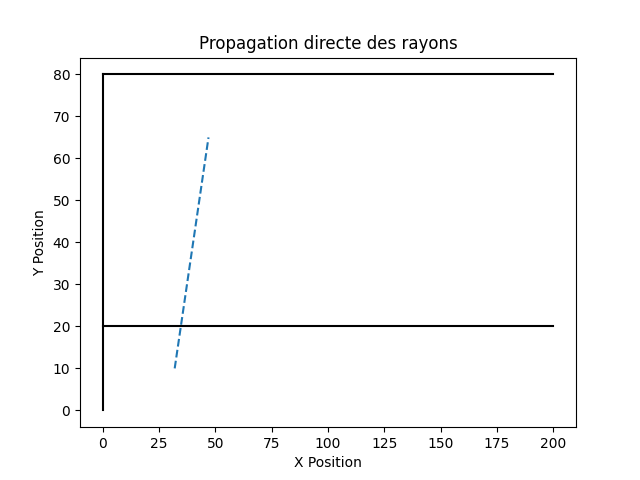
\includegraphics[width=0.8\textwidth]{Pictures/propa_dir.png}
    \caption{Propagation directe exercice 4.1}
    \label{fig:propd}
\end{figure}
\begin{figure}[H]
    \centering
    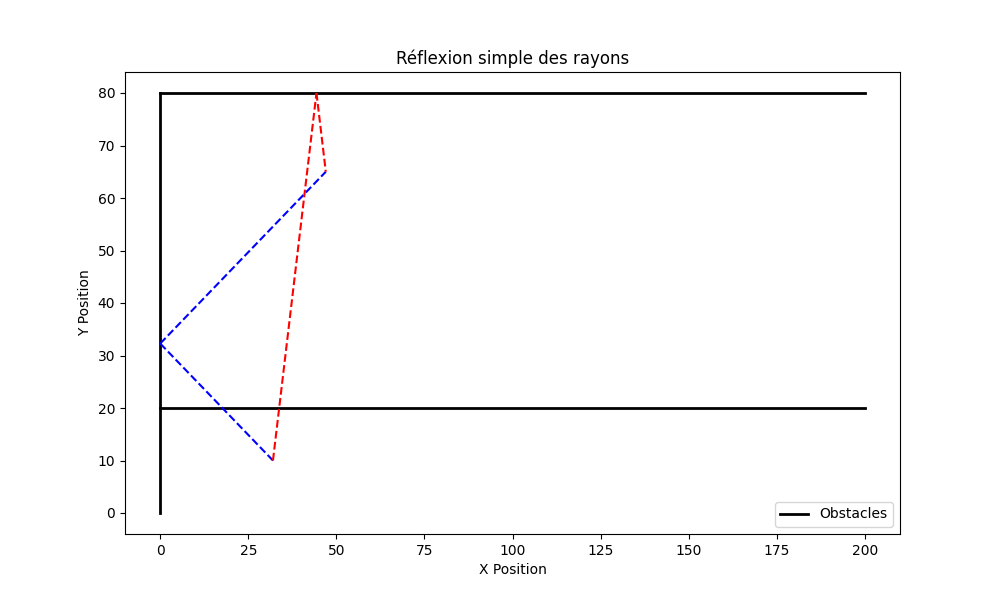
\includegraphics[width=0.8\textwidth]{Pictures/simple_reflex.png}
    \caption{réflexions simples exercice 4.1}
    \label{refs}
\end{figure}
\begin{figure}[H]
    \centering
    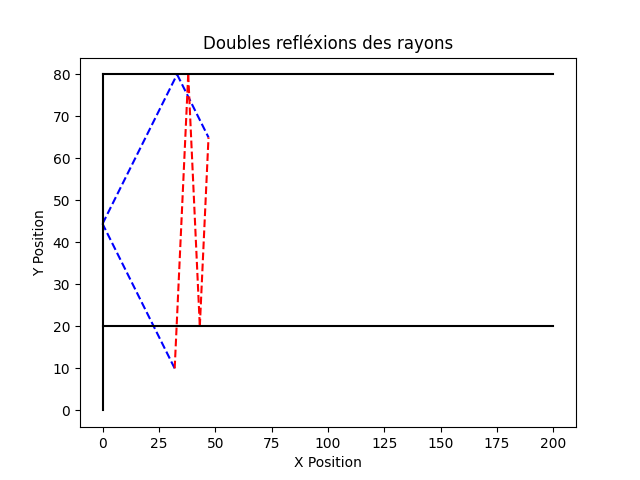
\includegraphics[width=0.8\textwidth]{Pictures/double_reflex.png}
    \caption{réflexions doubles exercice 4.1}
    \label{refd}
\end{figure}
\begin{figure}[H]
    \centering
    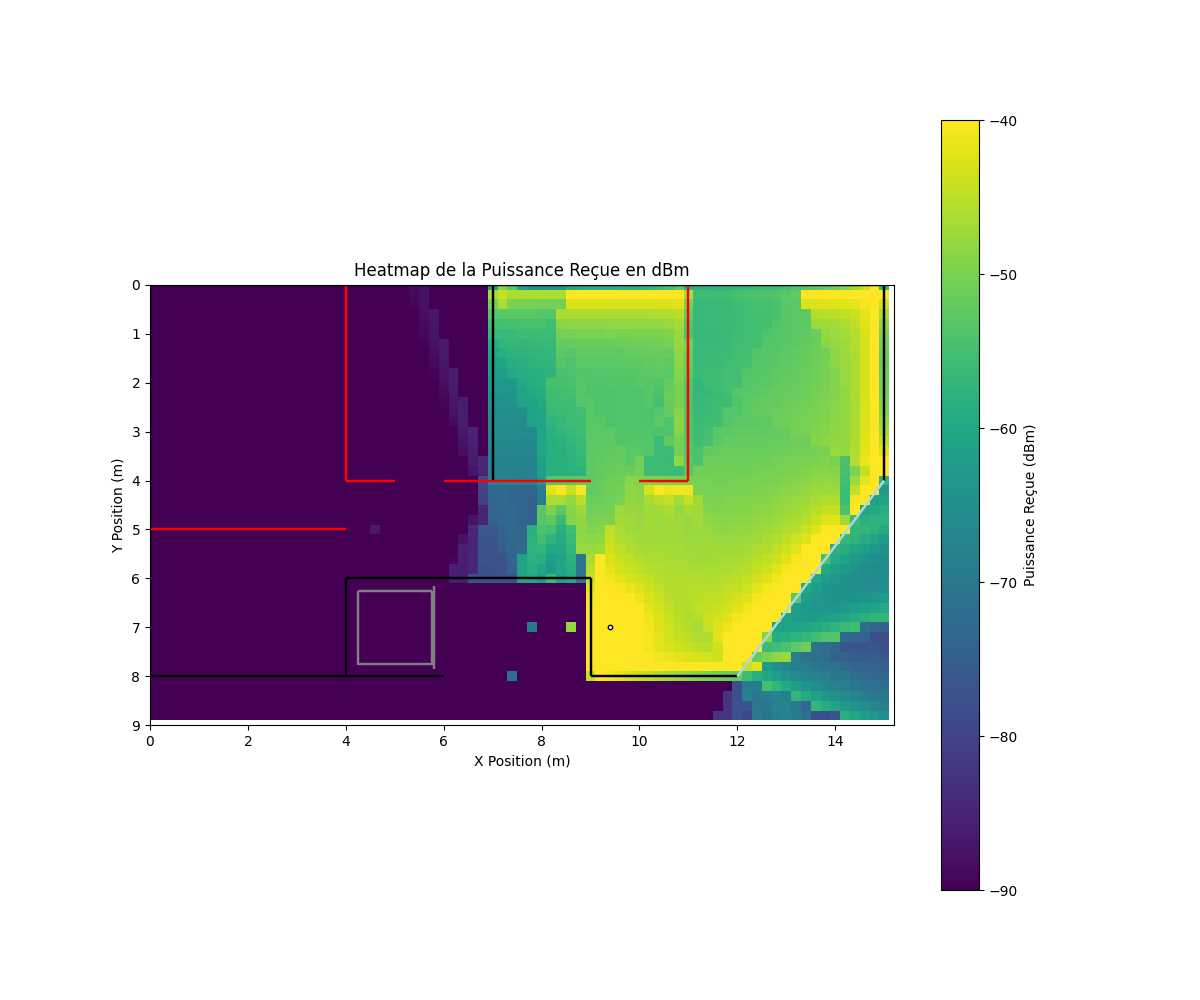
\includegraphics[width=0.8\textwidth]{Pictures/dBm.png}
    \caption{Puissance, Scénario de base avec ascenceur}
    \label{dbmbasea}
\end{figure}
\begin{figure}[H]
    \centering
    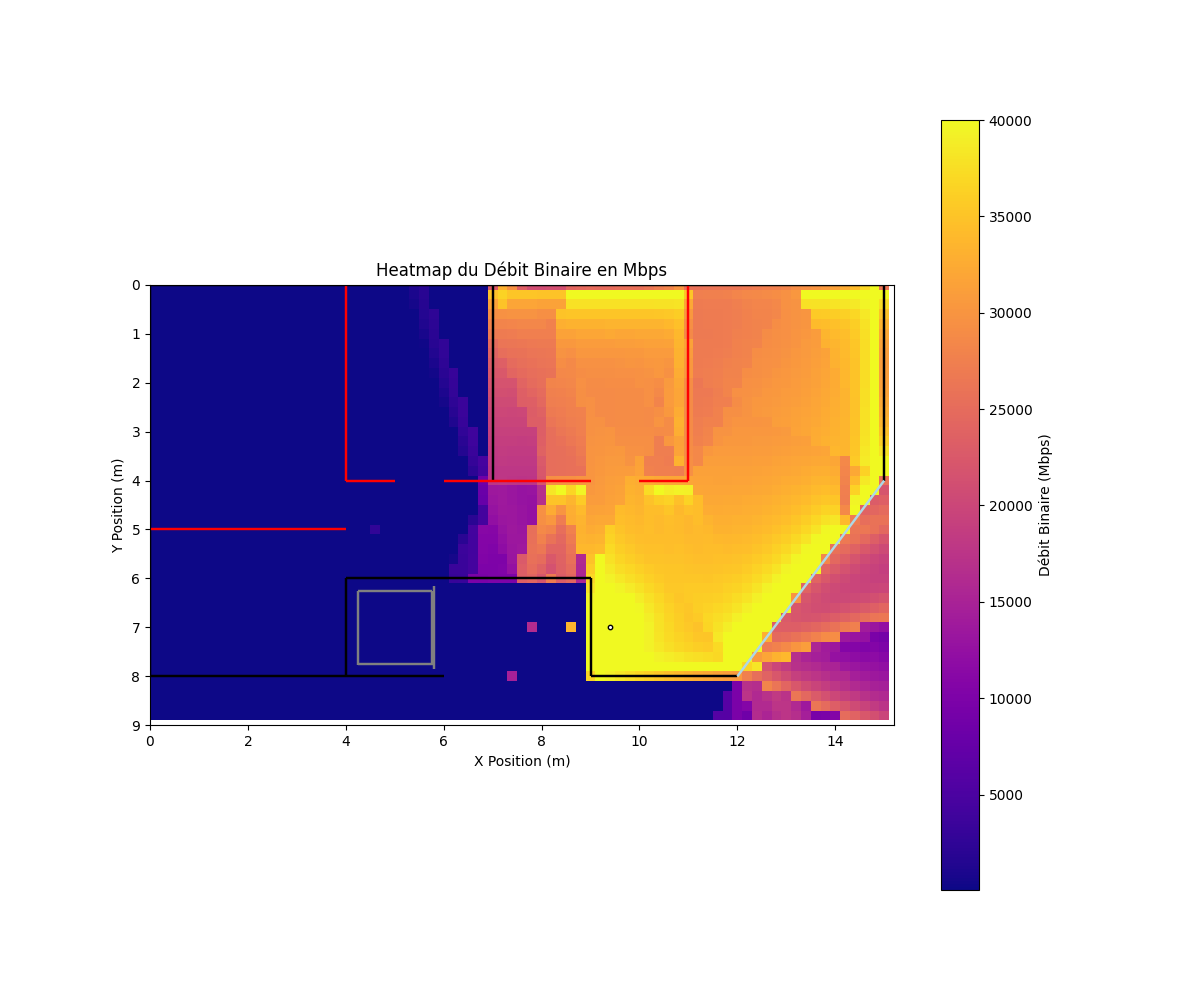
\includegraphics[width=0.8\textwidth]{Pictures/mbps.png}
    \caption{Débit Binaire, Scénario de base avec ascenceur}
    \label{mbpsbasea}
\end{figure}
\begin{figure}[H]
    \centering
    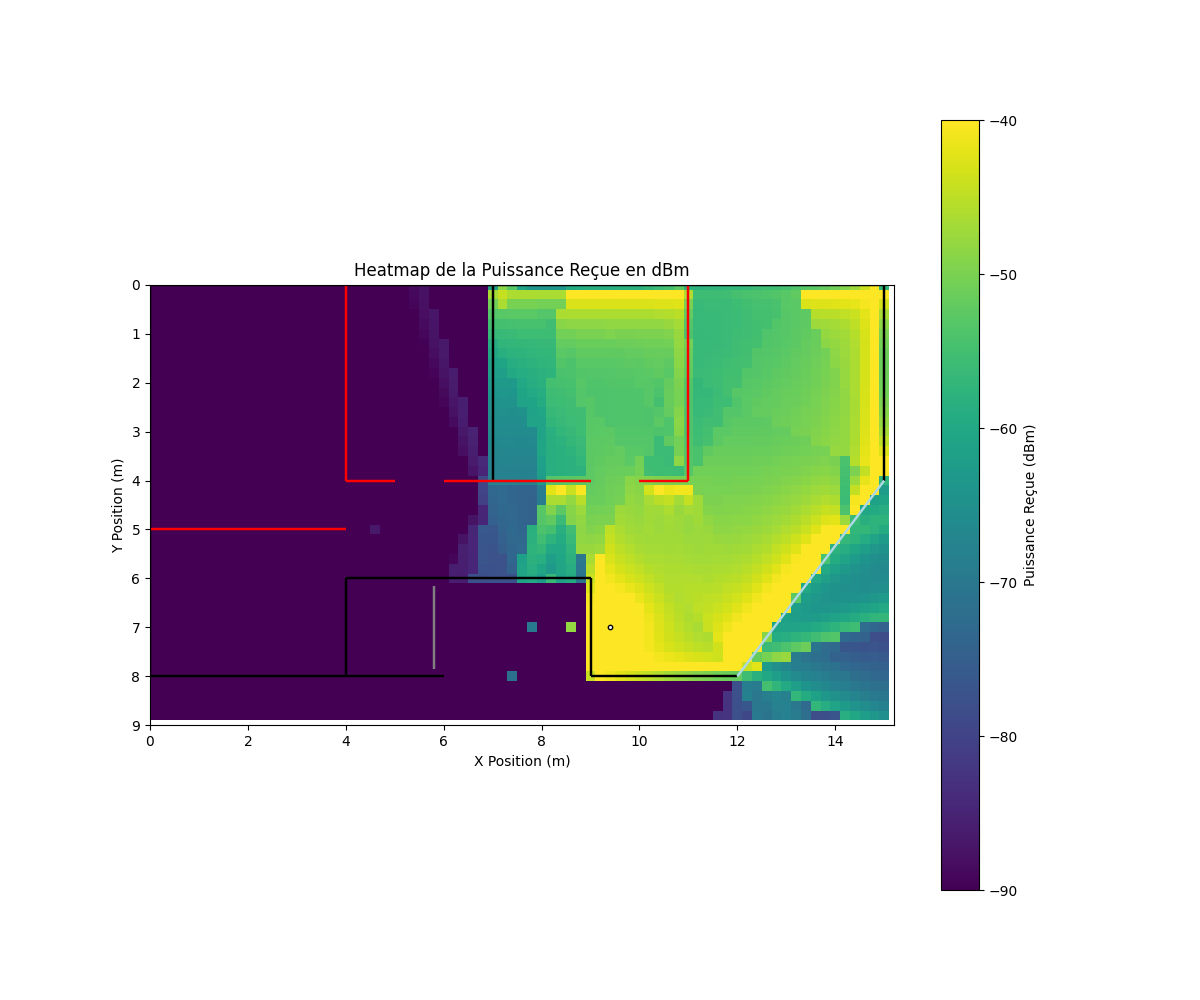
\includegraphics[width=0.8\textwidth]{Pictures/bpmsa.png}
    \caption{Puissance, Scénario de base sans ascenceur}
    \label{dbmbasesa}
\end{figure}
\begin{figure}[H]
    \centering
    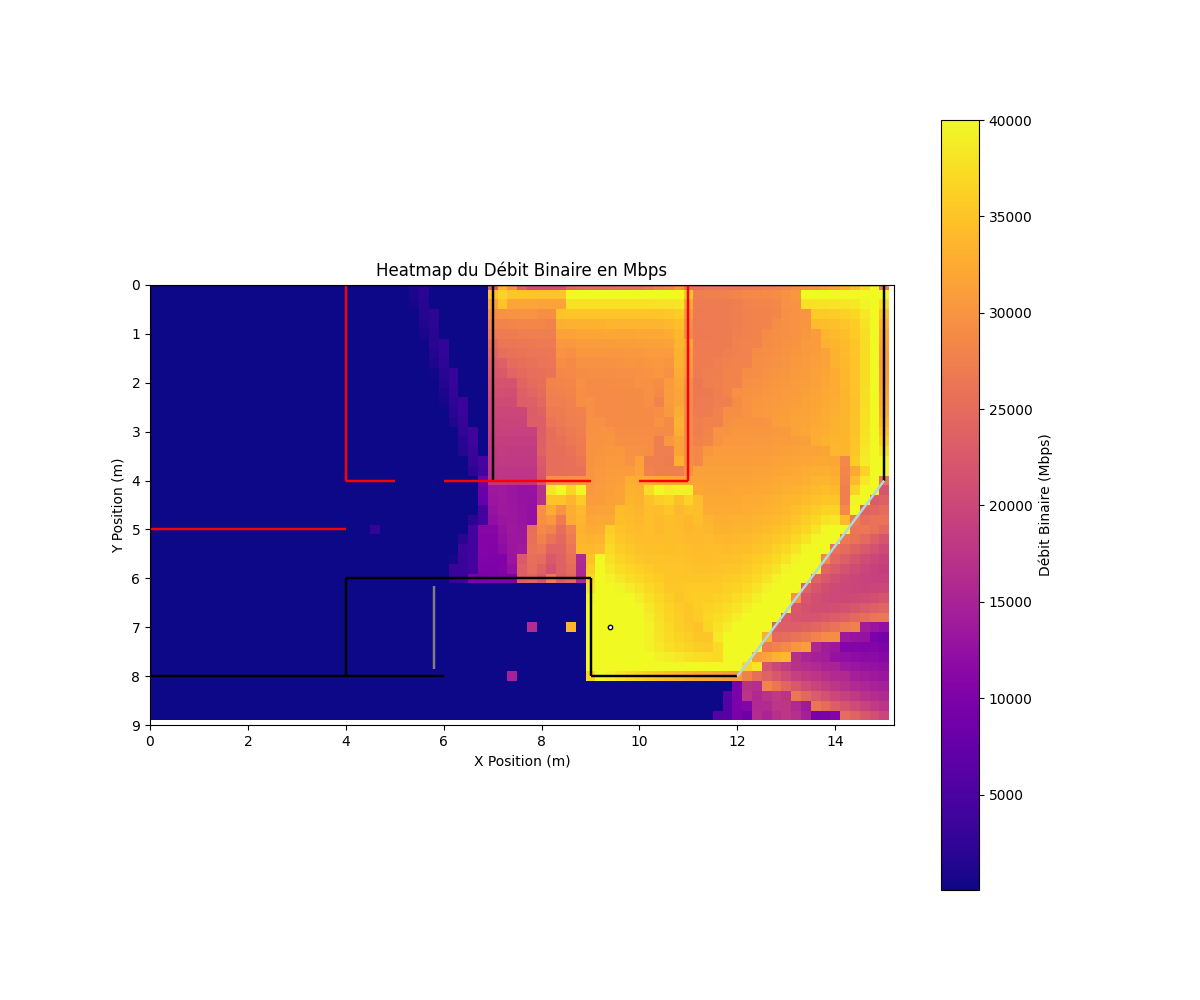
\includegraphics[width=0.8\textwidth]{Pictures/mbpssa.png}
    \caption{Débit Binaire, Scénario de base sans ascenceur}
    \label{mbpsbasesa}
\end{figure}
\begin{figure}[H]
    \centering
    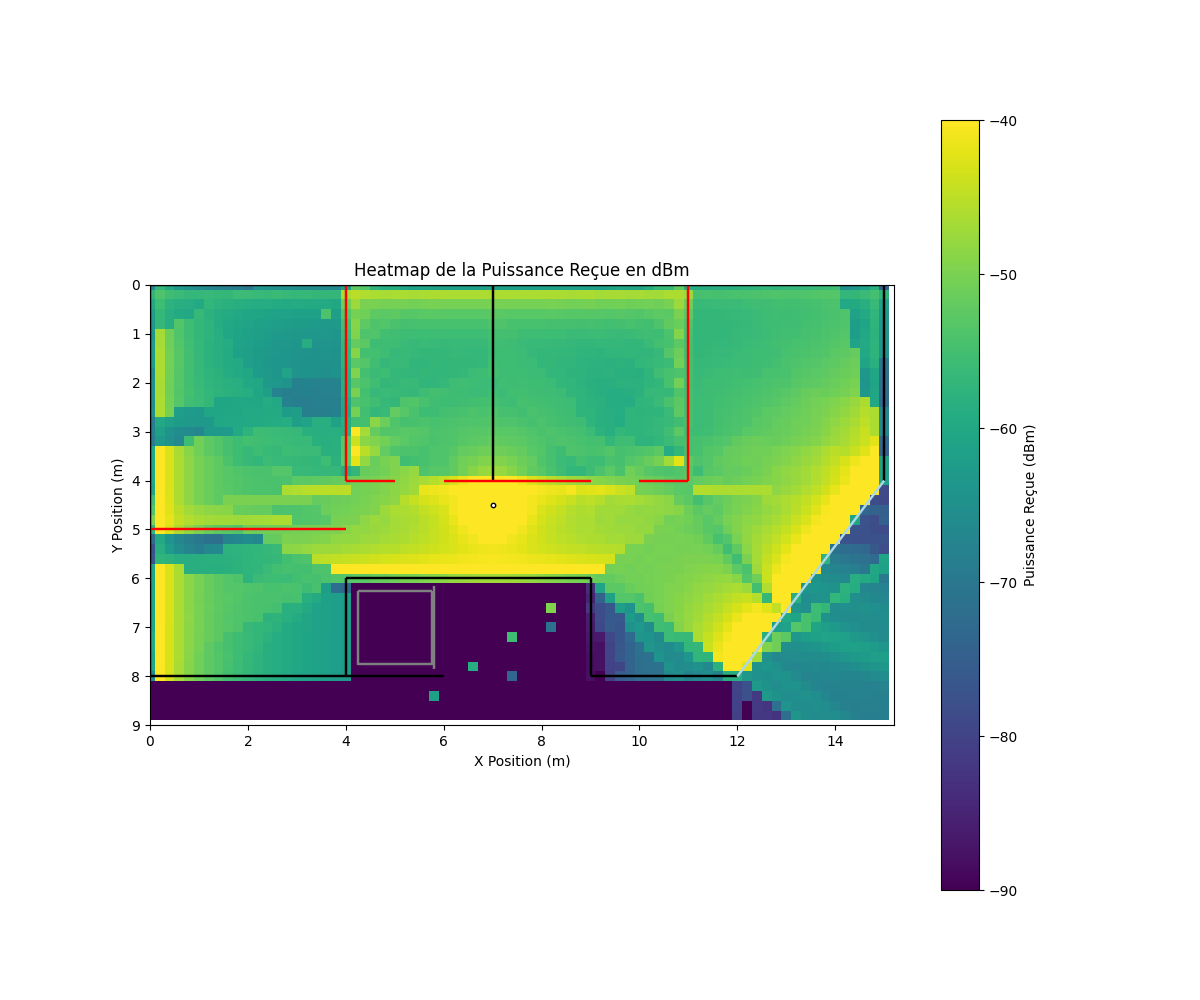
\includegraphics[width=0.8\textwidth]{Pictures/opt1bpma.png}
    \caption{Puissance, Optimisation avec 1 émetteur en (7, -4.5) avec ascenseur }
    \label{opti1adbm}
\end{figure}
\begin{figure}[H]
    \centering
    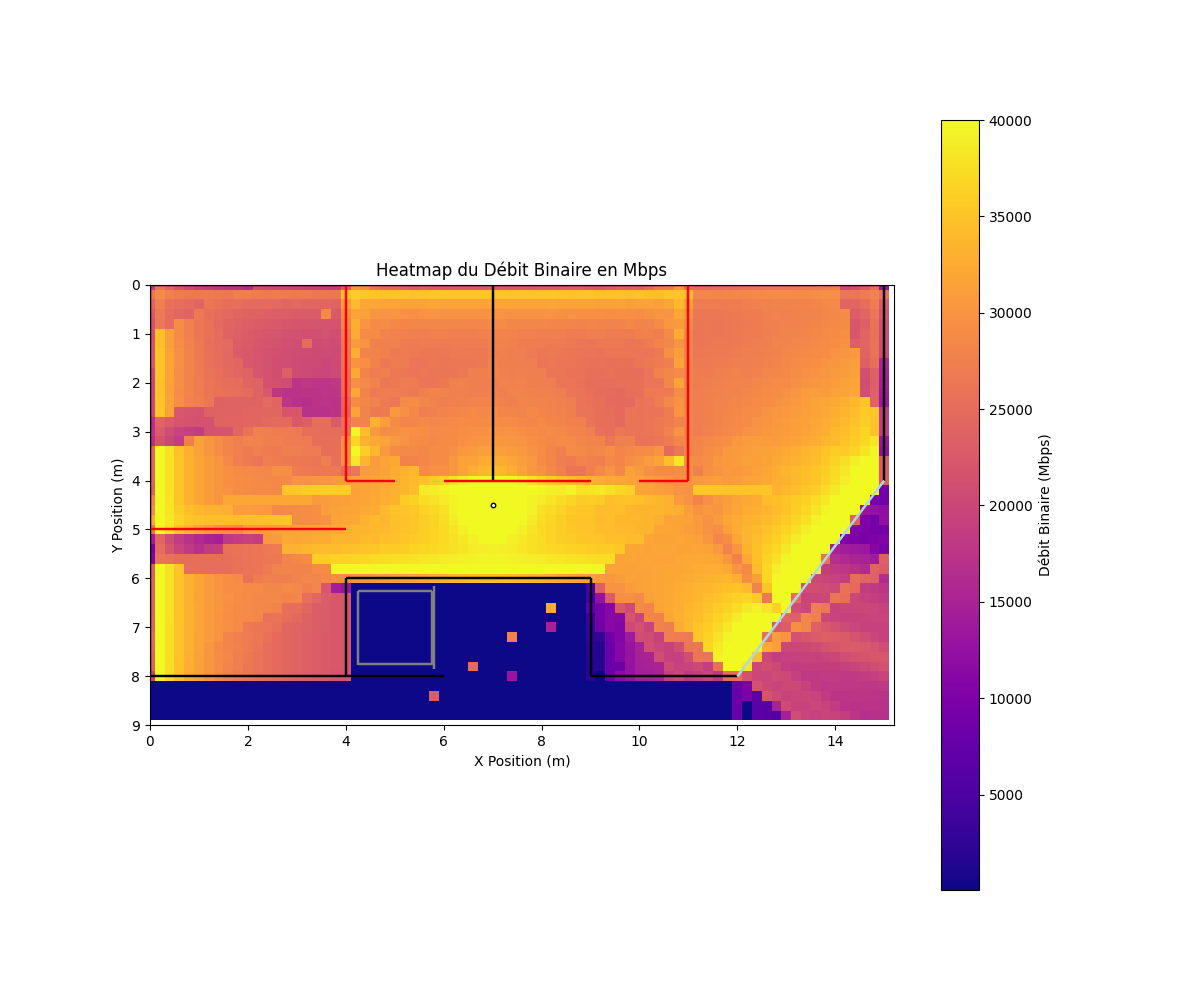
\includegraphics[width=0.8\textwidth]{Pictures/opti1mbpsa.png}
    \caption{Débit Binaire, Optimisation avec 1 émetteur en (7, -4.5) avec ascenseur}
    \label{opti1ambps}
\end{figure}
\begin{figure}[H]
    \centering
    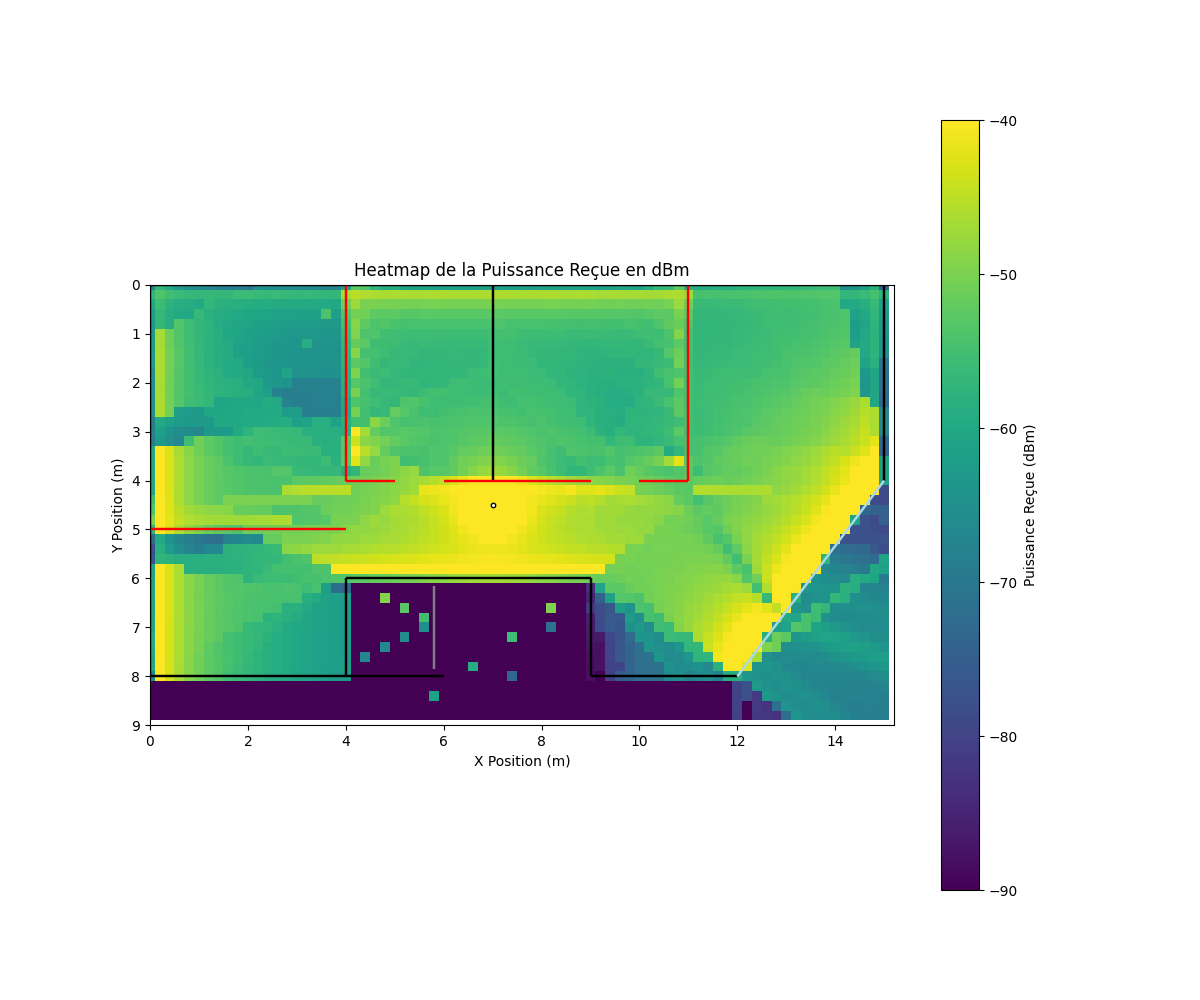
\includegraphics[width=0.8\textwidth]{Pictures/opt1bpm.png}
    \caption{Puissance, Optimisation avec 1 émetteur en (7, -4.5) sans ascenseur}
    \label{opti1dbm}
\end{figure}
\begin{figure}[H]
    \centering
    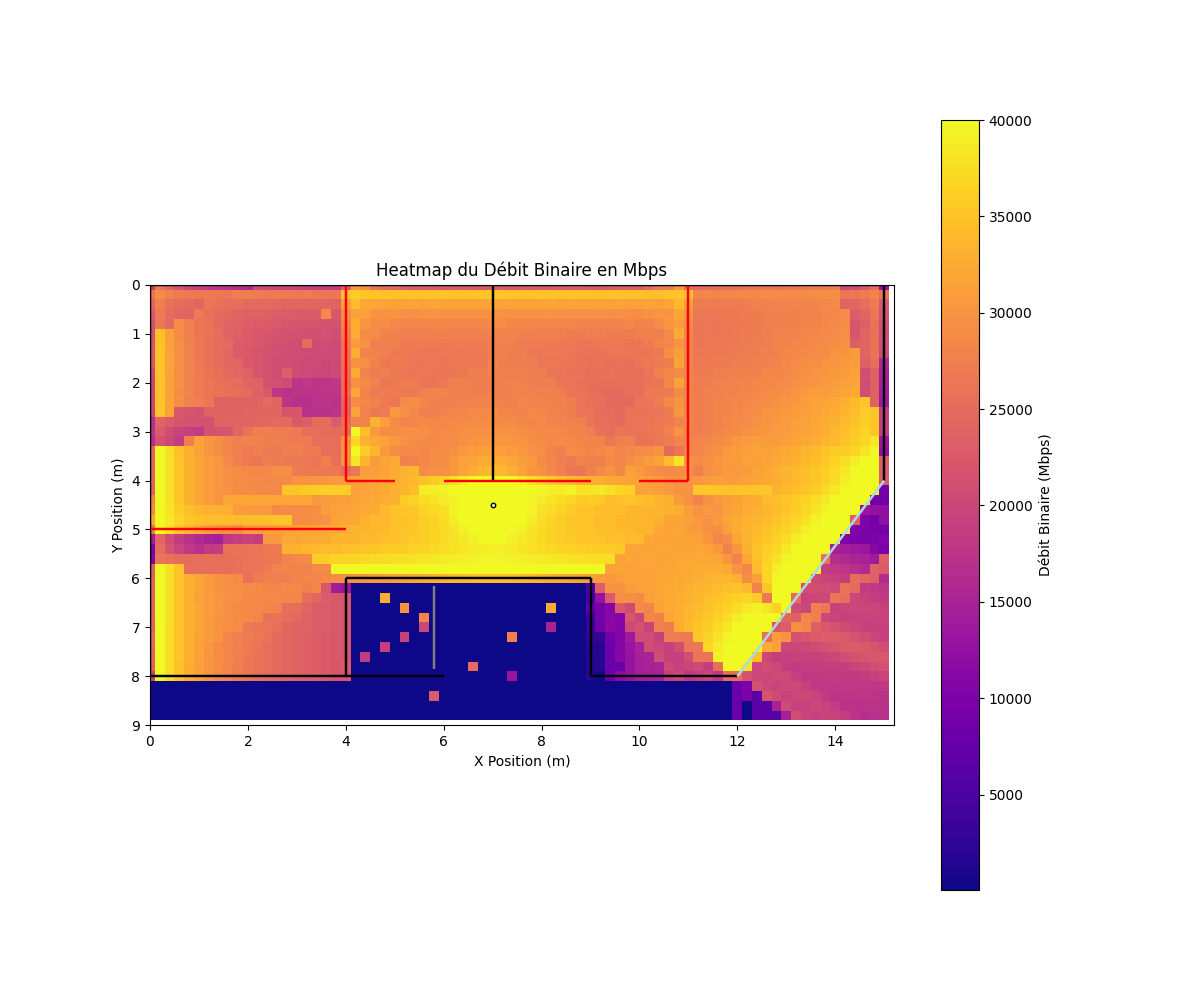
\includegraphics[width=0.8\textwidth]{Pictures/opti1mbps.png}
    \caption{Débit Binaire, Optimisation avec 1 émetteur en (7, -4.5) sans ascenseur}
    \label{opti1mbps}
\end{figure}
\begin{figure}[H]
    \centering
    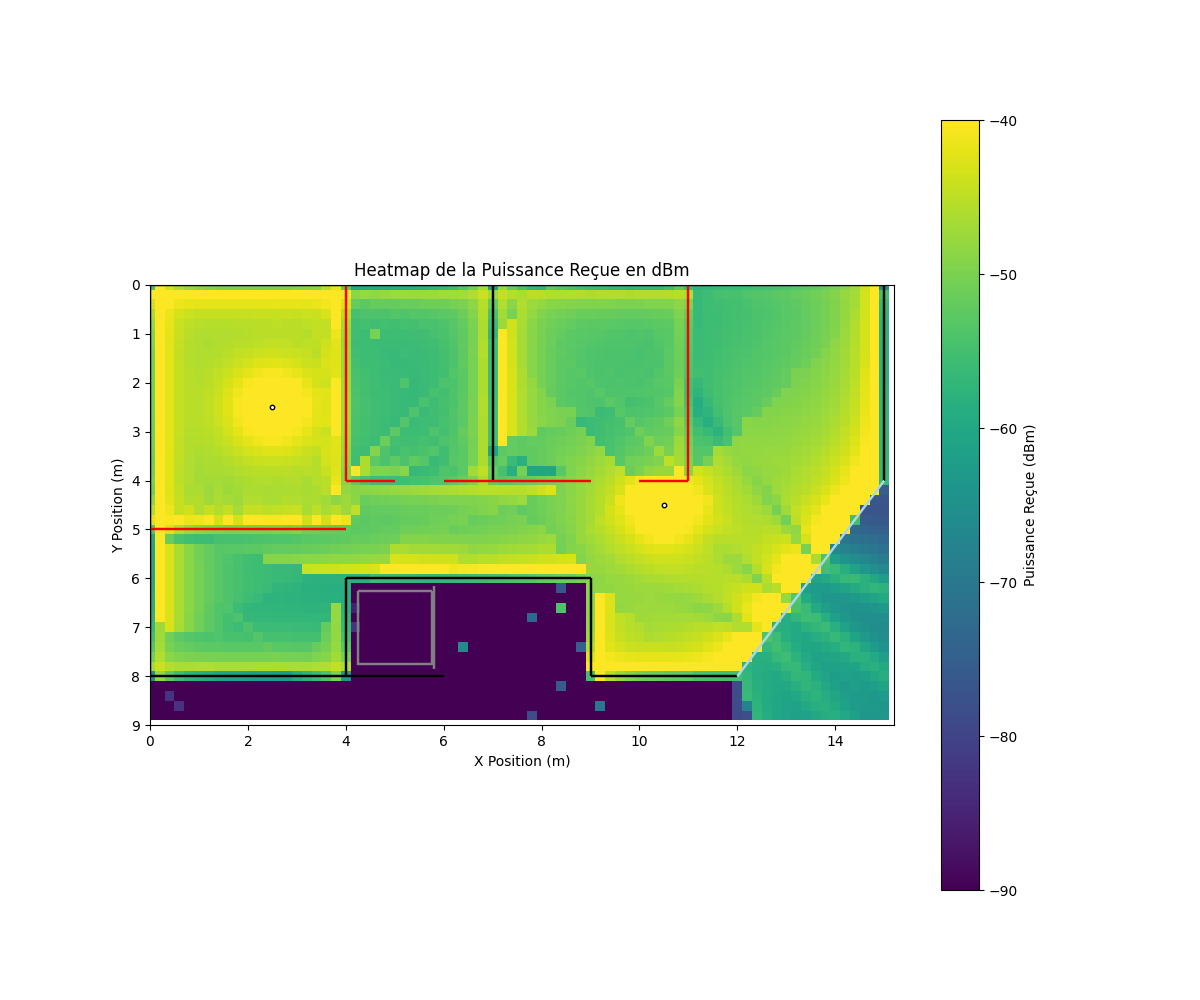
\includegraphics[width=0.8\textwidth]{Pictures/opti2dbma.png}
    \caption{Puissance, Optimisation avec  émetteurs en (2.5, -2.5) et (10.5, -4.5) avec ascenseur}
    \label{opti2dbma}
\end{figure}
\begin{figure}[H]
    \centering
    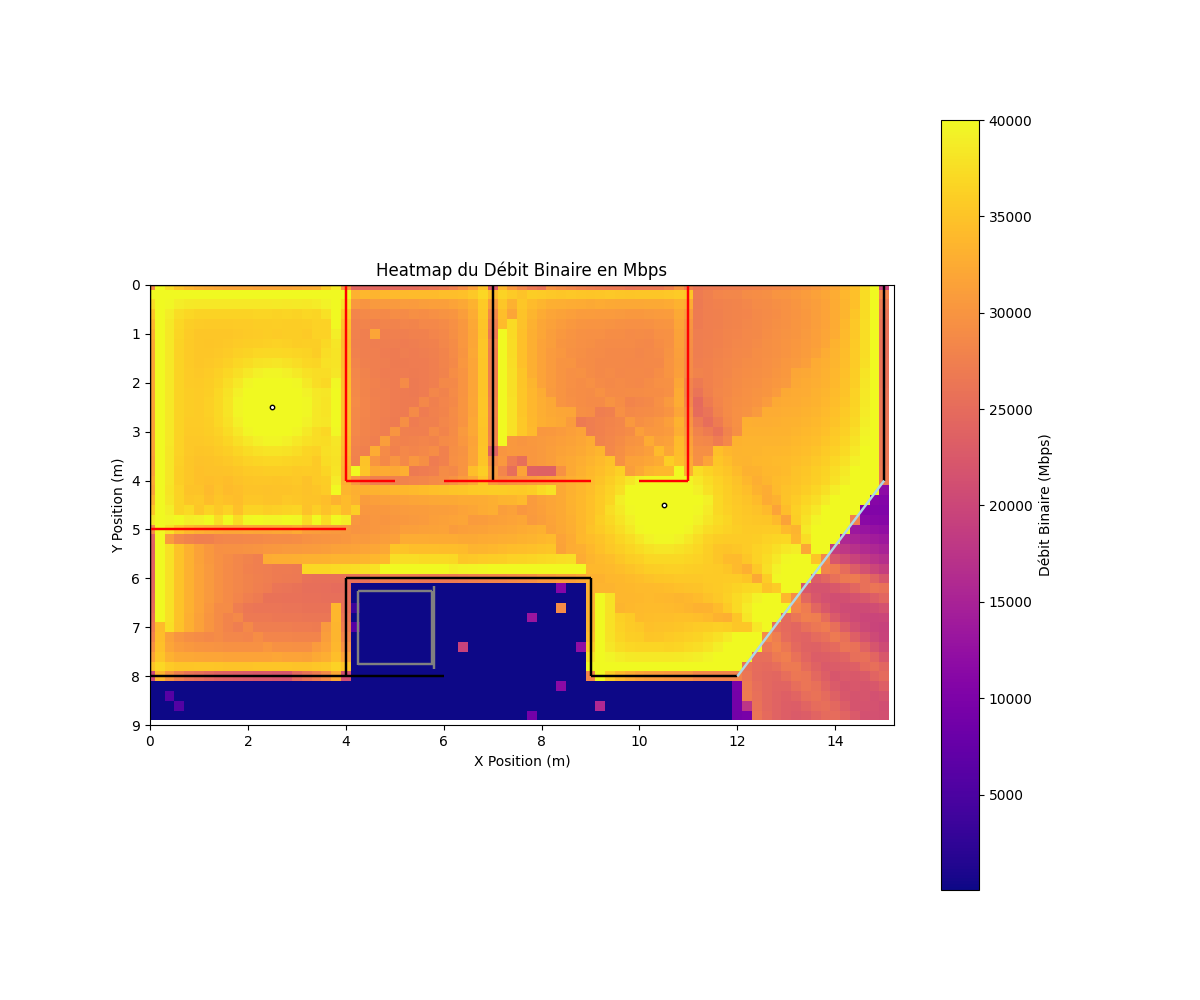
\includegraphics[width=0.8\textwidth]{Pictures/opti2mbpsa.png}
    \caption{Débit Binaire, Optimisation avec 2 émetteurs en (2.5, -2.5) et (10.5, -4.5) avec ascenseur}
    \label{opti2mbpsa}
\end{figure}
\begin{figure}[H]
    \centering
    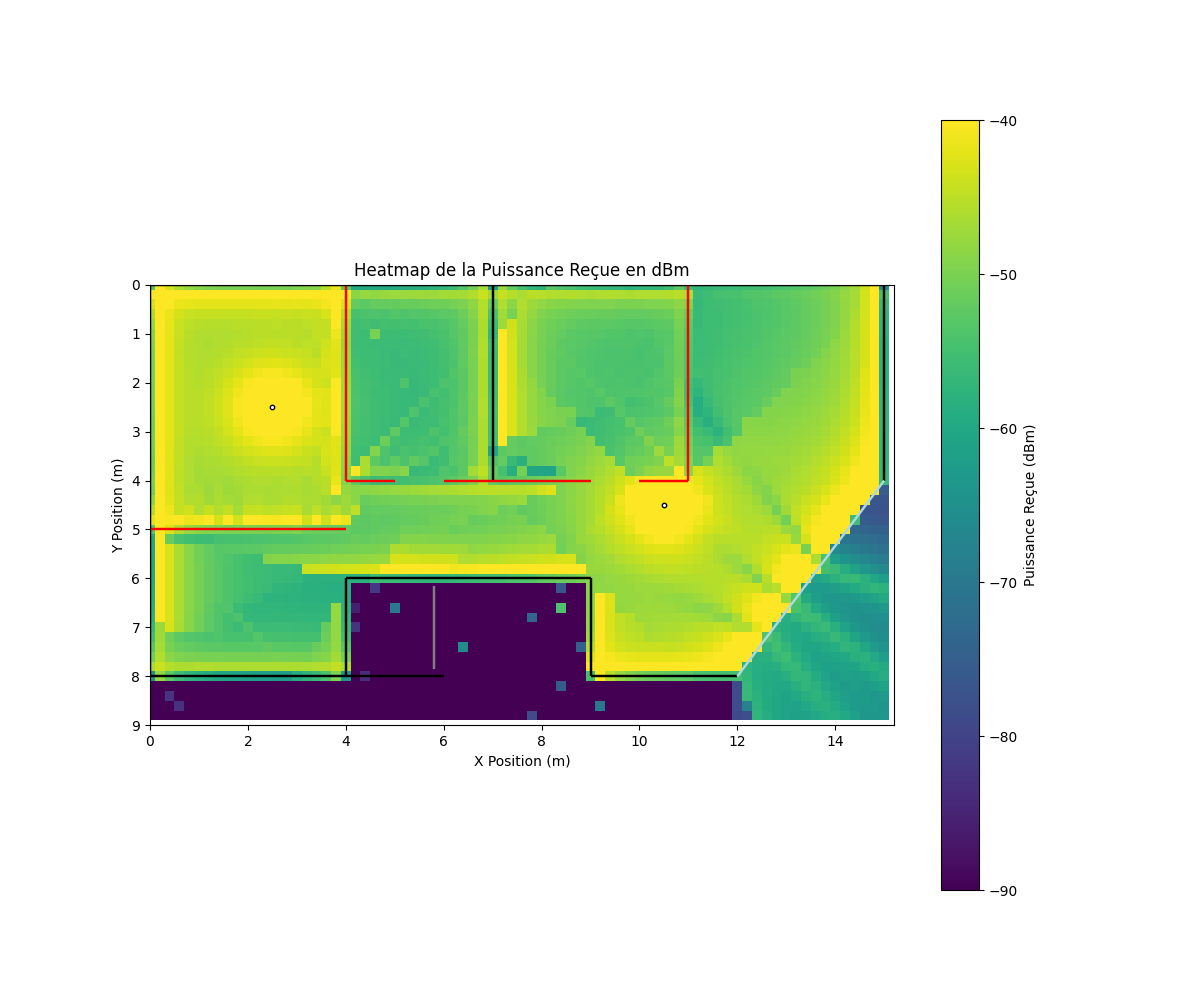
\includegraphics[width=0.8\textwidth]{Pictures/opti2dbm.png}
    \caption{Puissance, Optimisation avec 2 émetteurs en (2.5, -2.5) et (10.5, -4.5) sans ascenseur}
    \label{opti2dbm}
\end{figure}
\begin{figure}[H]
    \centering
    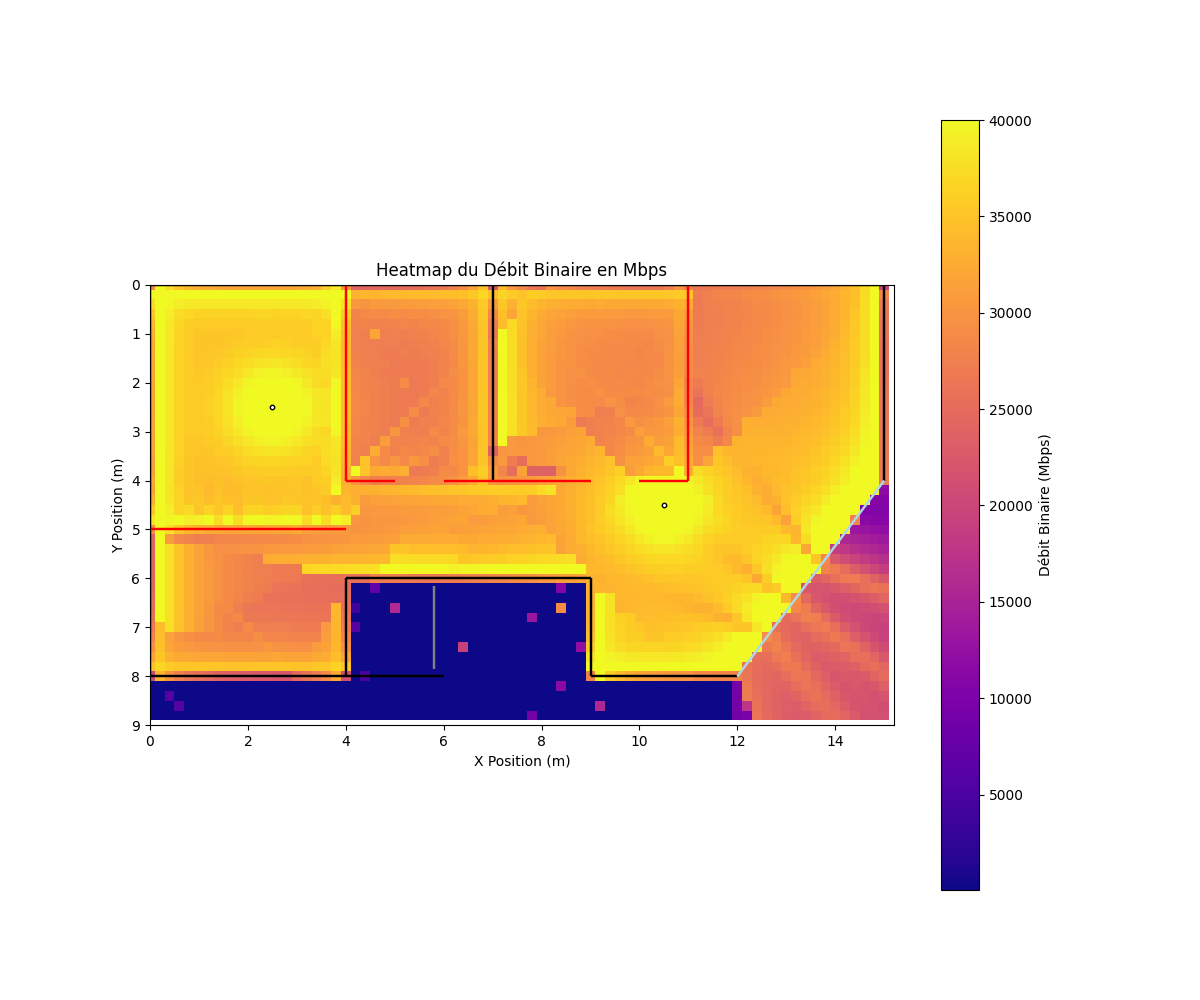
\includegraphics[width=0.8\textwidth]{Pictures/opti2mbps.png}
    \caption{Débit Binaire, Optimisation avec 2 émetteurs en (2.5, -2.5) et (10.5, -4.5) sans ascenseur}
    \label{opti2mbps}
\end{figure}
    \chapter{Code Source}
    \label{codesource}
    \subsection*{Environment.py}
\inputminted[linenos, breaklines]{python}{Python/environment.py}

\subsection*{RayTracing.py}
\inputminted[linenos, breaklines]{python}{Python/raytracing2.py}

\subsection*{Physics.py}
\inputminted[linenos, breaklines]{python}{Python/physics2.py}

\subsection*{Heatmap.py}
\inputminted[linenos, breaklines]{python}{Python/heatmap.py}

\subsection*{Optimisation.py}
\inputminted[linenos, breaklines]{python}{Python/optimisation.py}

\subsection*{Obstacle.py}
\inputminted[linenos, breaklines]{python}{Python/obstacle.py}

\subsection*{Emitter.py}
\inputminted[linenos, breaklines]{python}{Python/emitter.py}

\subsection*{Receiver.py}
\inputminted[linenos, breaklines]{python}{Python/receiver.py}

\subsection*{Position.py}
\inputminted[linenos, breaklines]{python}{Python/position.py}

\subsection*{Material.py}
\inputminted[linenos, breaklines]{python}{Python/material.py}



\end{appendices}

\end{document}